\documentclass[xcolor=dvipsnames]{beamer}
\usetheme{nelle}
\usepackage{natbib}                 % Fancy bibliography.
\usepackage{url}                    % Allow printing of URLs.
\usepackage{outlines}
\usepackage{enumitem}
\usepackage{multicol}
\usepackage{dsfont}
\usepackage{amsmath}
\usepackage{epstopdf}
\usepackage{color}
\setbeamerfont{caption}{size=\scriptsize}
\setbeamertemplate{navigation symbols}{}
\setbeamertemplate{footline}[frame number]{}

\def\newblock{\hskip .11em plus .33em minus .07em}

\title{\textbf{Hi-C data and meta-genomic}}

\author[Varoquaux Nelle]{
Nelle Varoquaux}


\date{December, 7th}
\institute{UC Berkeley, BIDS}
\begin{document}
\begin{frame}[t, noframenumbering]
  \maketitle

\end{frame}

\setcounter{framenumber}{0}

\section{Introduction}
% 1. Why?
\begin{frame}
\frametitle{The 3D structure of the genome is thought to play an important
role in many biological processes}
\vspace{-0.6em}
\begin{figure}
\begin{center}
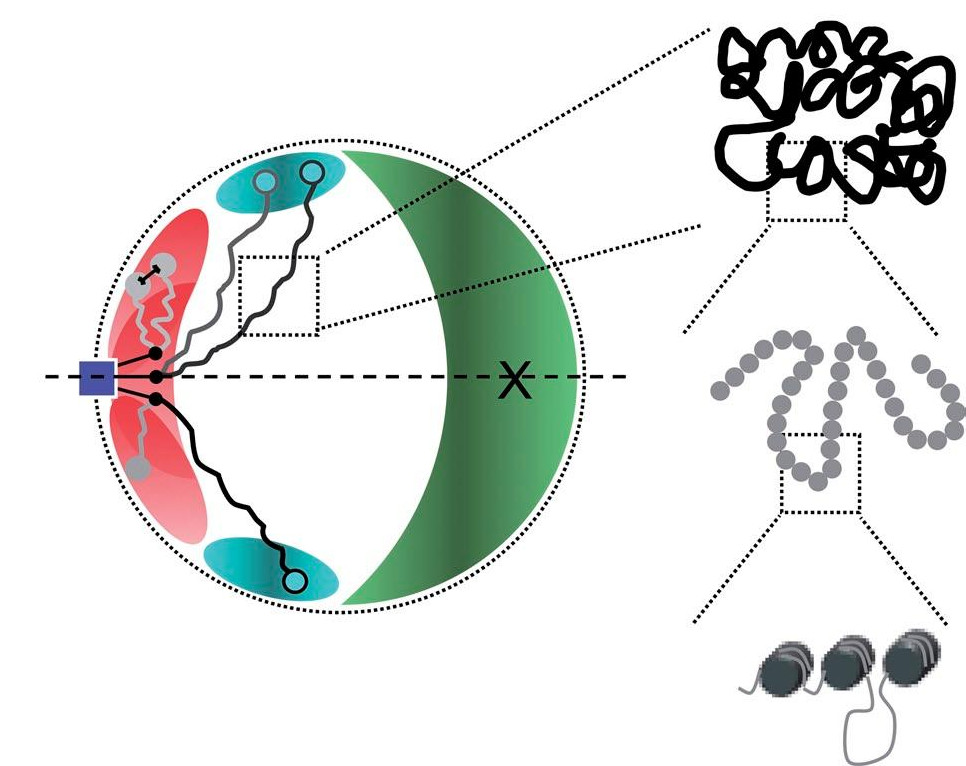
\includegraphics[width=0.7\linewidth]{figures/yeasts_genome_architecture.jpg}
\end{center}
\caption{\textbf{The genome of \textit{S. cerevisiae} is highly organized}
         \citep{zimmer:principles}}
\end{figure}
\end{frame}

% 2. What is the Hi-C protocol?
\begin{frame}
\frametitle{The Hi-C protocol identifies physical contacts between
pairs of loci genome-wide}
\begin{figure}
\centering
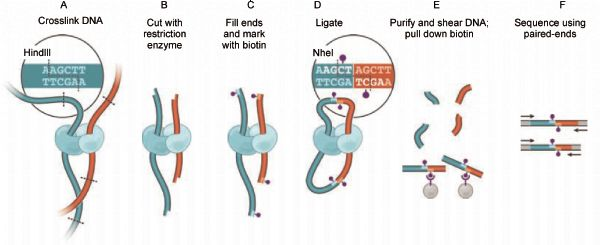
\includegraphics[width=0.85\textwidth]{figures/hic_protocol.jpg}
\caption{\textbf{Hi-C paves the way for a systematic and genome-wide analysis
of genome architecture} \citep{rao:3d}}
\end{figure}
\end{frame}

% 3. A contact count matrix
\begin{frame}
\frametitle{The contact count matrix recapitulates the hallmarks of genome
architecture}
\vspace{-1em}
\begin{figure}
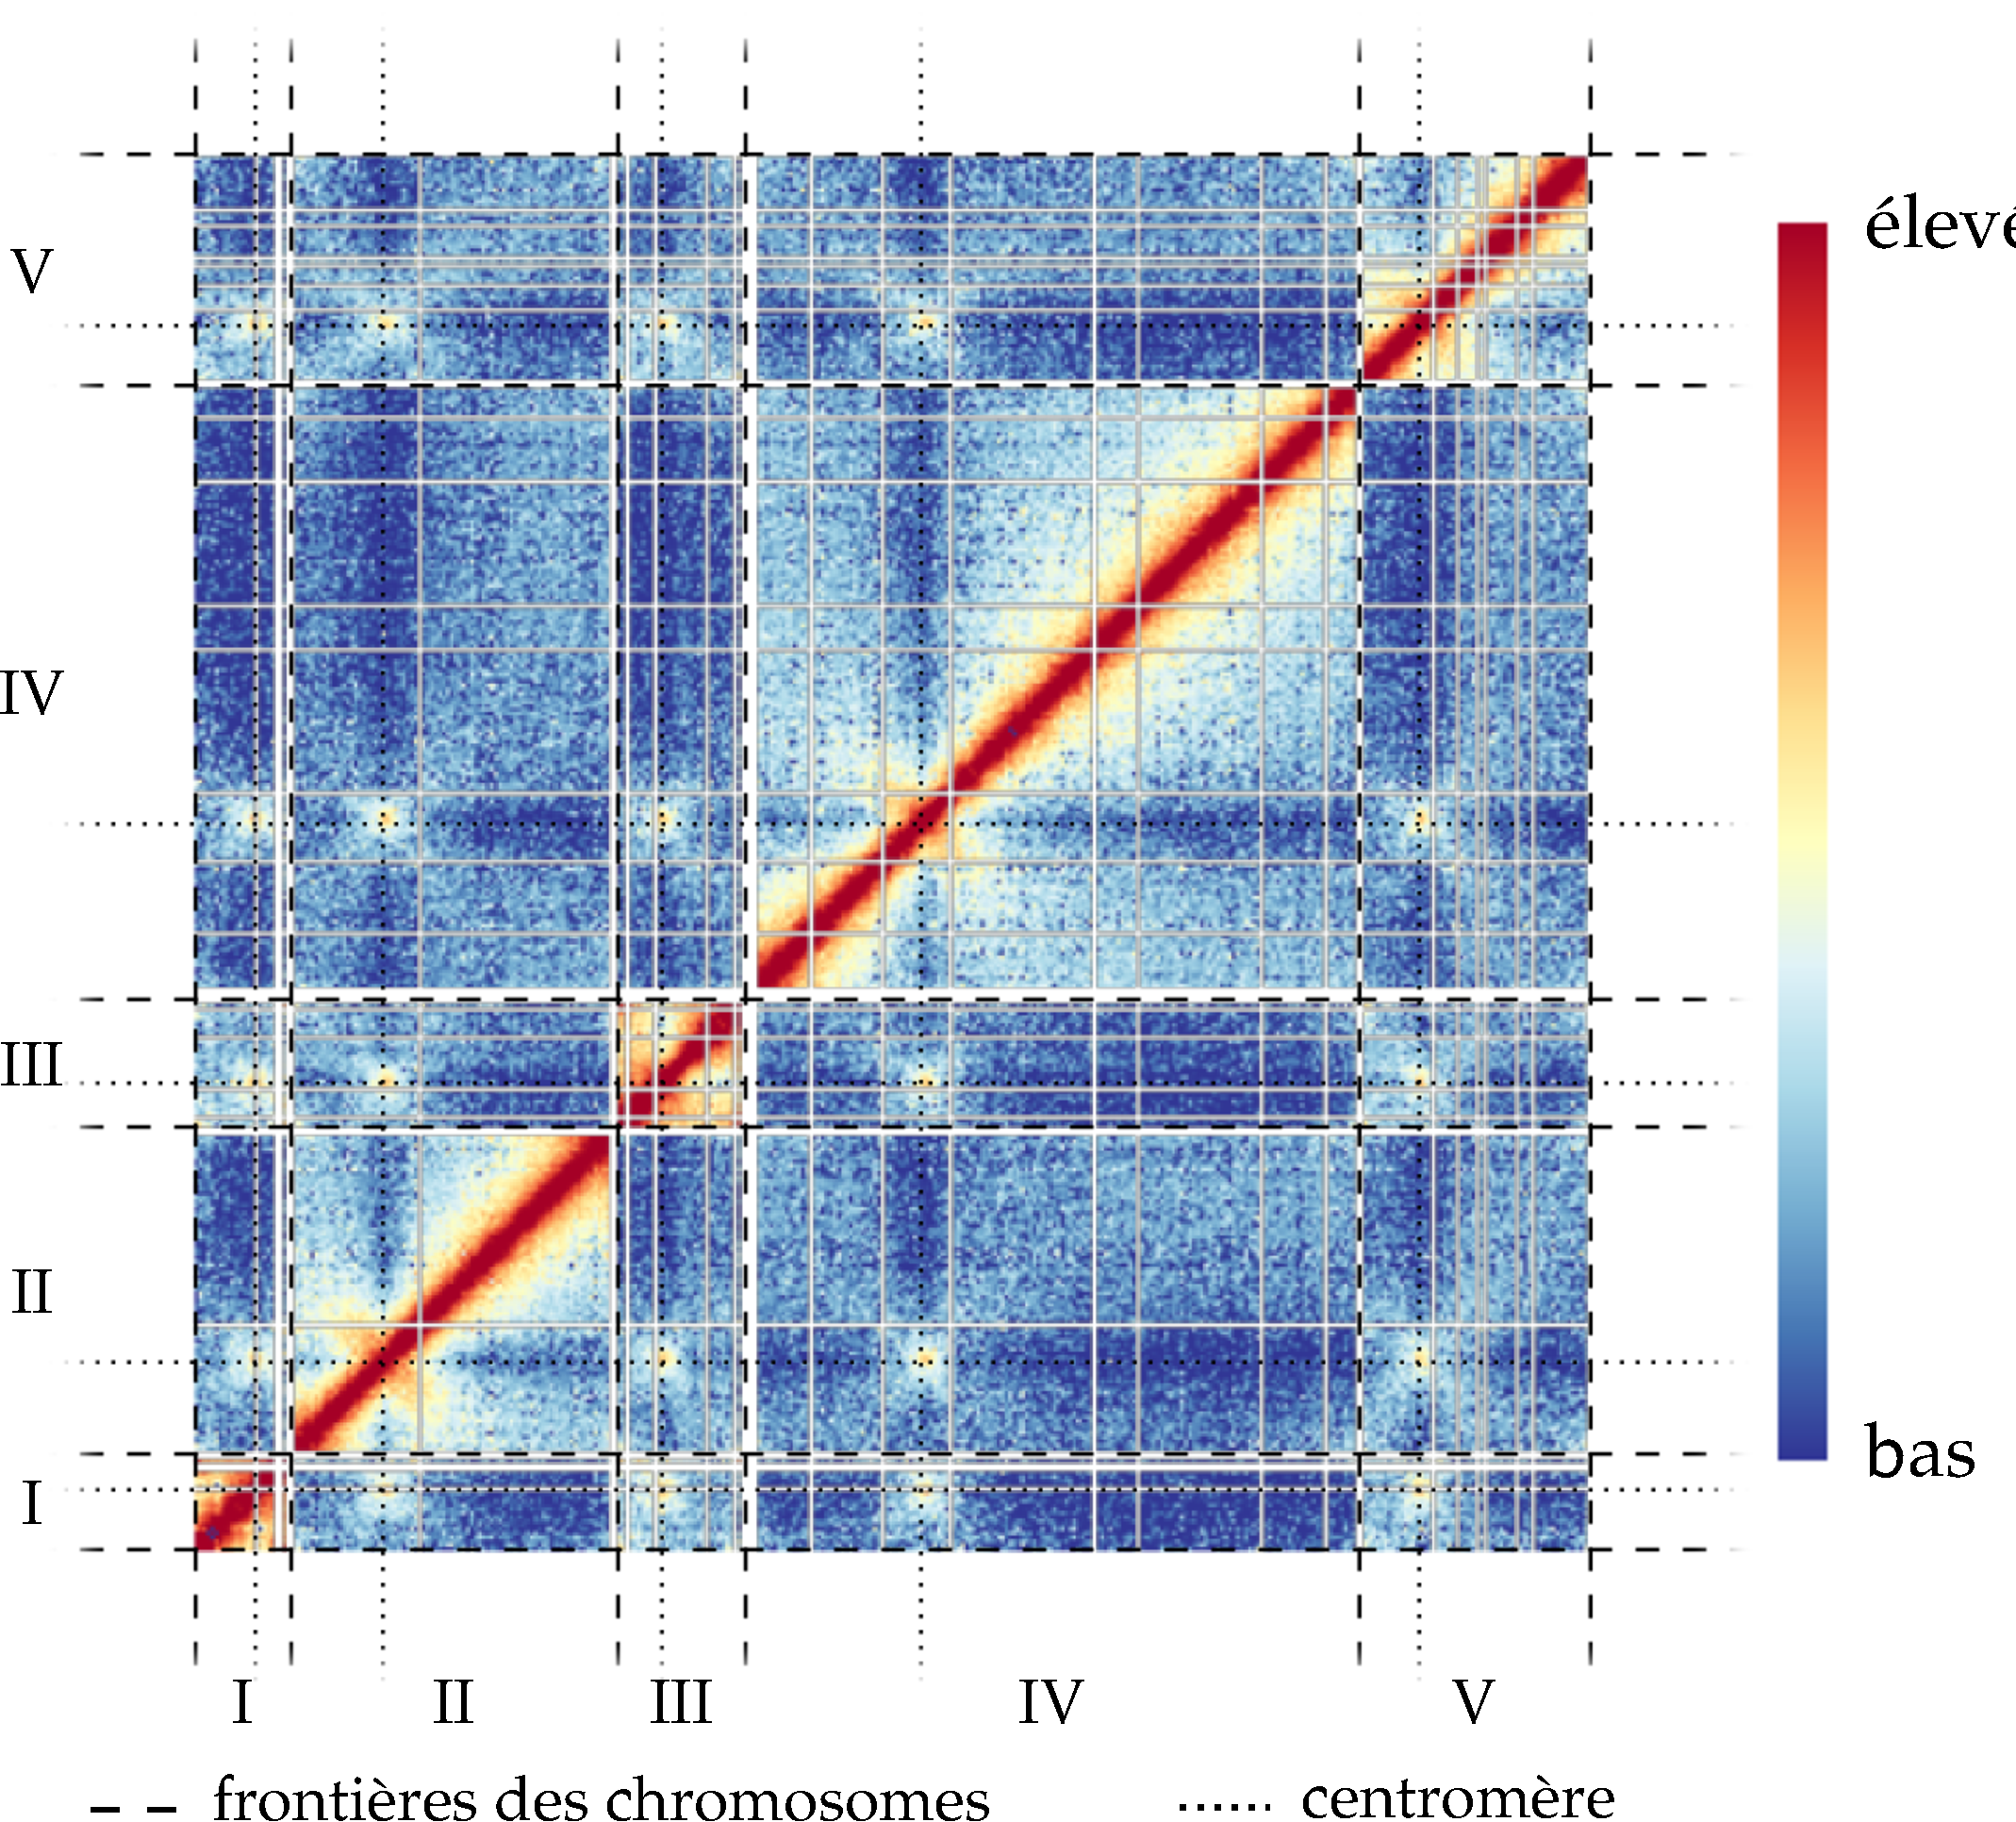
\includegraphics[width=0.55\textwidth]{figures/yeast_counts.pdf}
\caption{\textbf{Contact counts for the first 5 chromosomes of \textit{S.
cerevisiae}}}
\end{figure}
\end{frame}

\begin{frame}
\frametitle{HiC-Pro: from sequences to contact maps}
\begin{figure}
\begin{center}
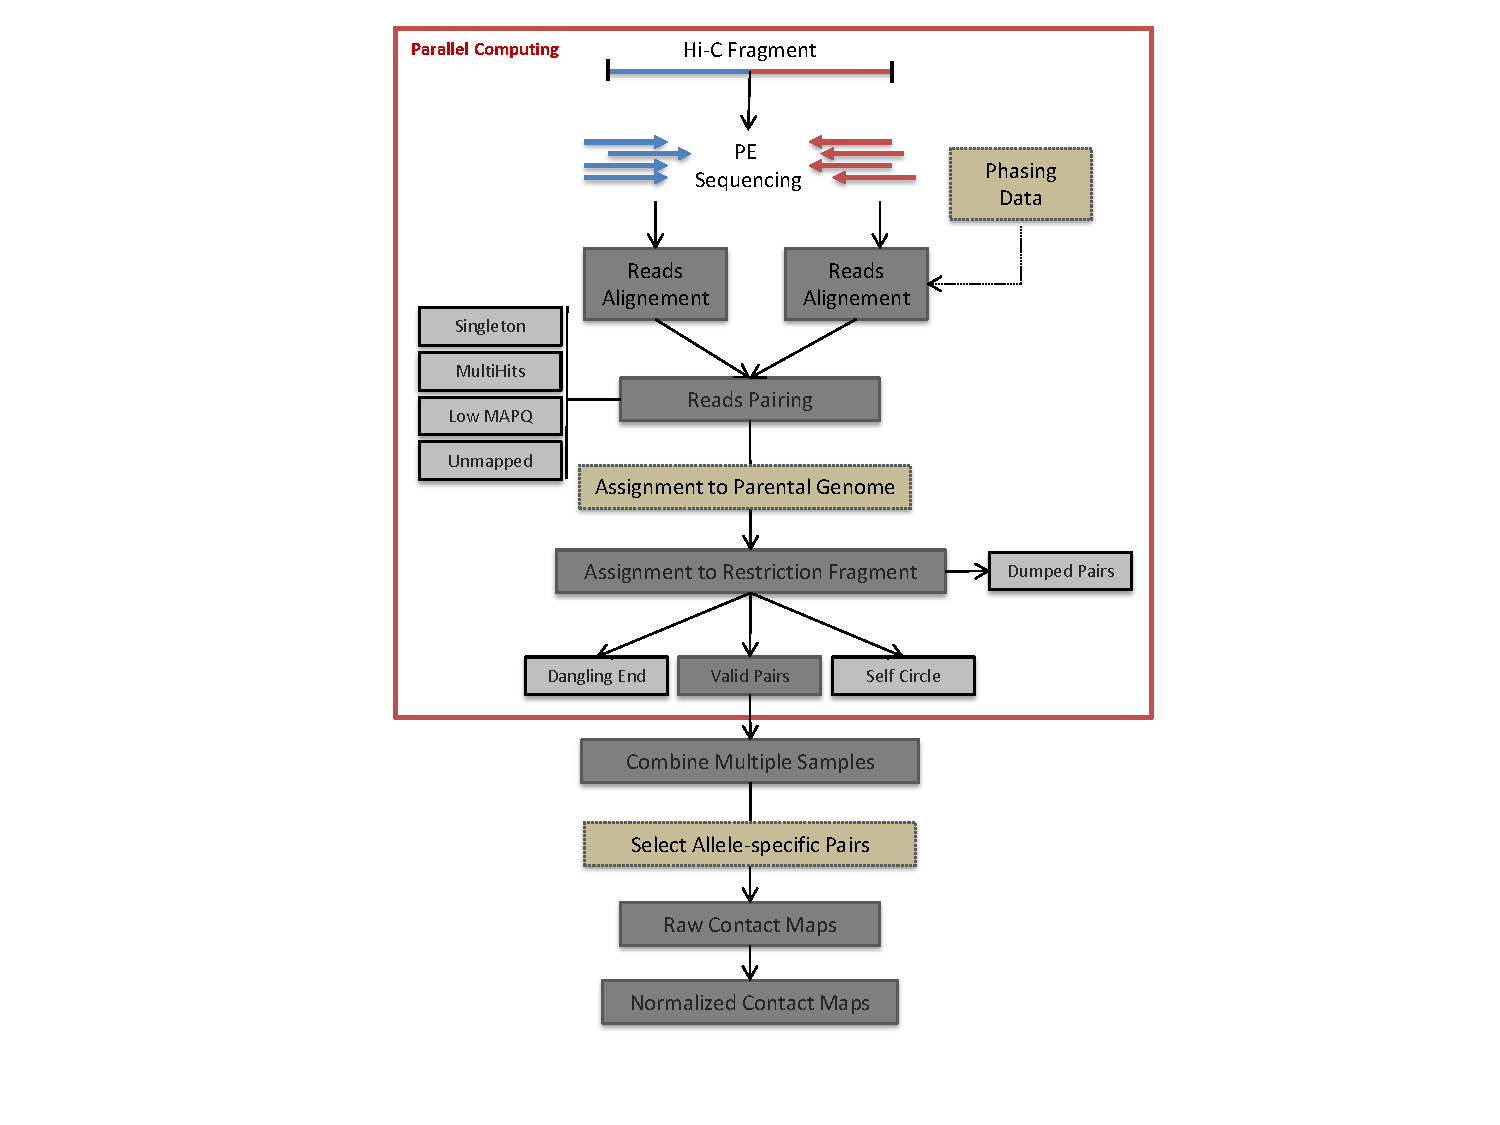
\includegraphics[width=0.9\linewidth]{figures/hic-pro.pdf}
\end{center}
\end{figure}
\end{frame}

\begin{frame}
\frametitle{A wide range of applications for Hi-C data}
\begin{overlayarea}{12cm}{6cm}
\begin{itemize}
\item<1-> \textbf{Studying the 3D structure of the genome}: 3D structure
inference, data integration with gene expression profiles, replication timing,
\dots
\item<2-> \textbf{Studying the 1D structure of the genome}: genome assembly,
metagenomic deconvolution, haplotype resolution, \dots
\item<3-> \textbf{Genome annotation}: identifying rDNA clusters, centromeres,
specific gene families, \dots
\end{itemize}
\end{overlayarea}
\begin{overlayarea}{12cm}{3cm}
\only<1>{
\vspace{-4cm}
\begin{center}
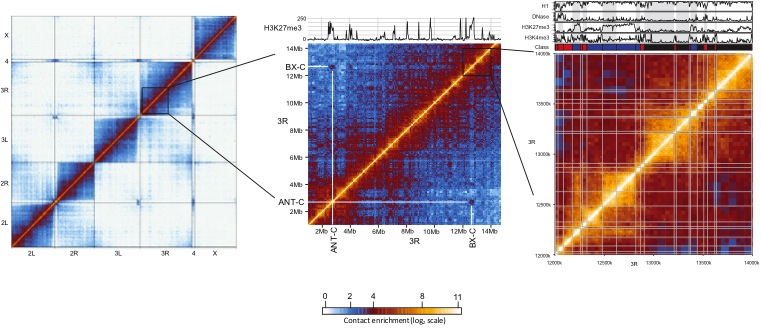
\includegraphics[width=0.9\linewidth]{figures/cavalli-illustration.jpg}
\end{center}}
\only<2>{
\vspace{-4cm}
\begin{center}
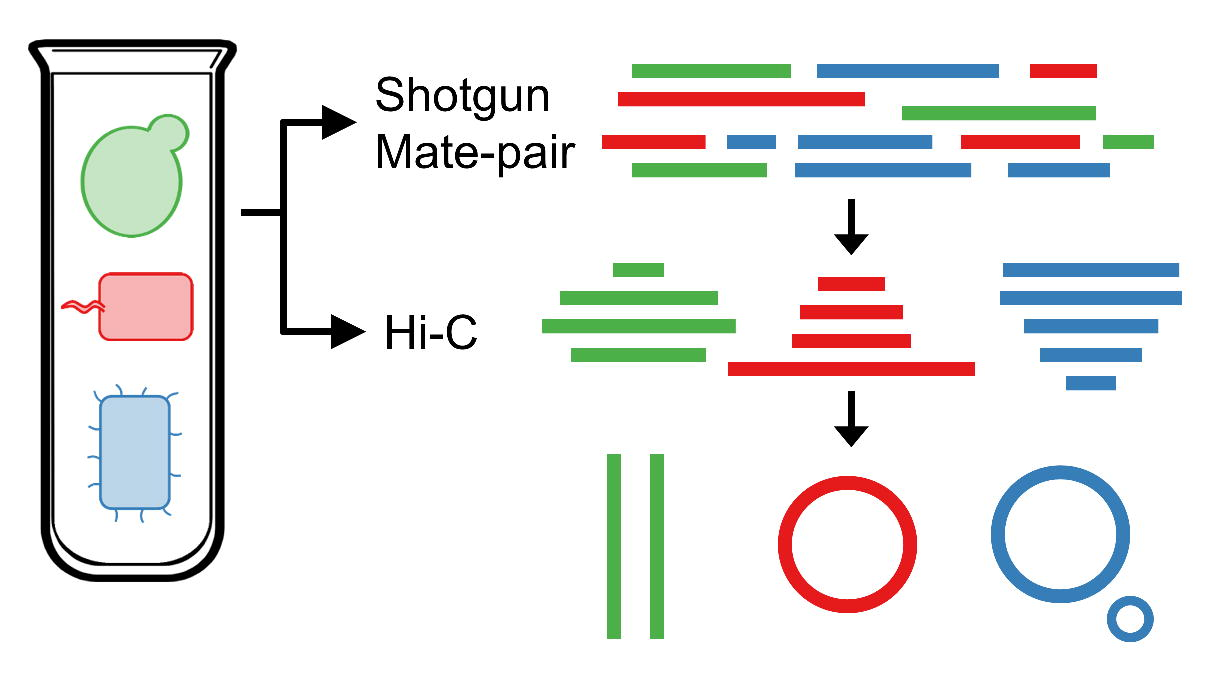
\includegraphics[width=0.75\linewidth]{figures/metagenomic_deconvolution.png}
\end{center}}
\only<3>{
\vspace{-3cm}
\begin{center}
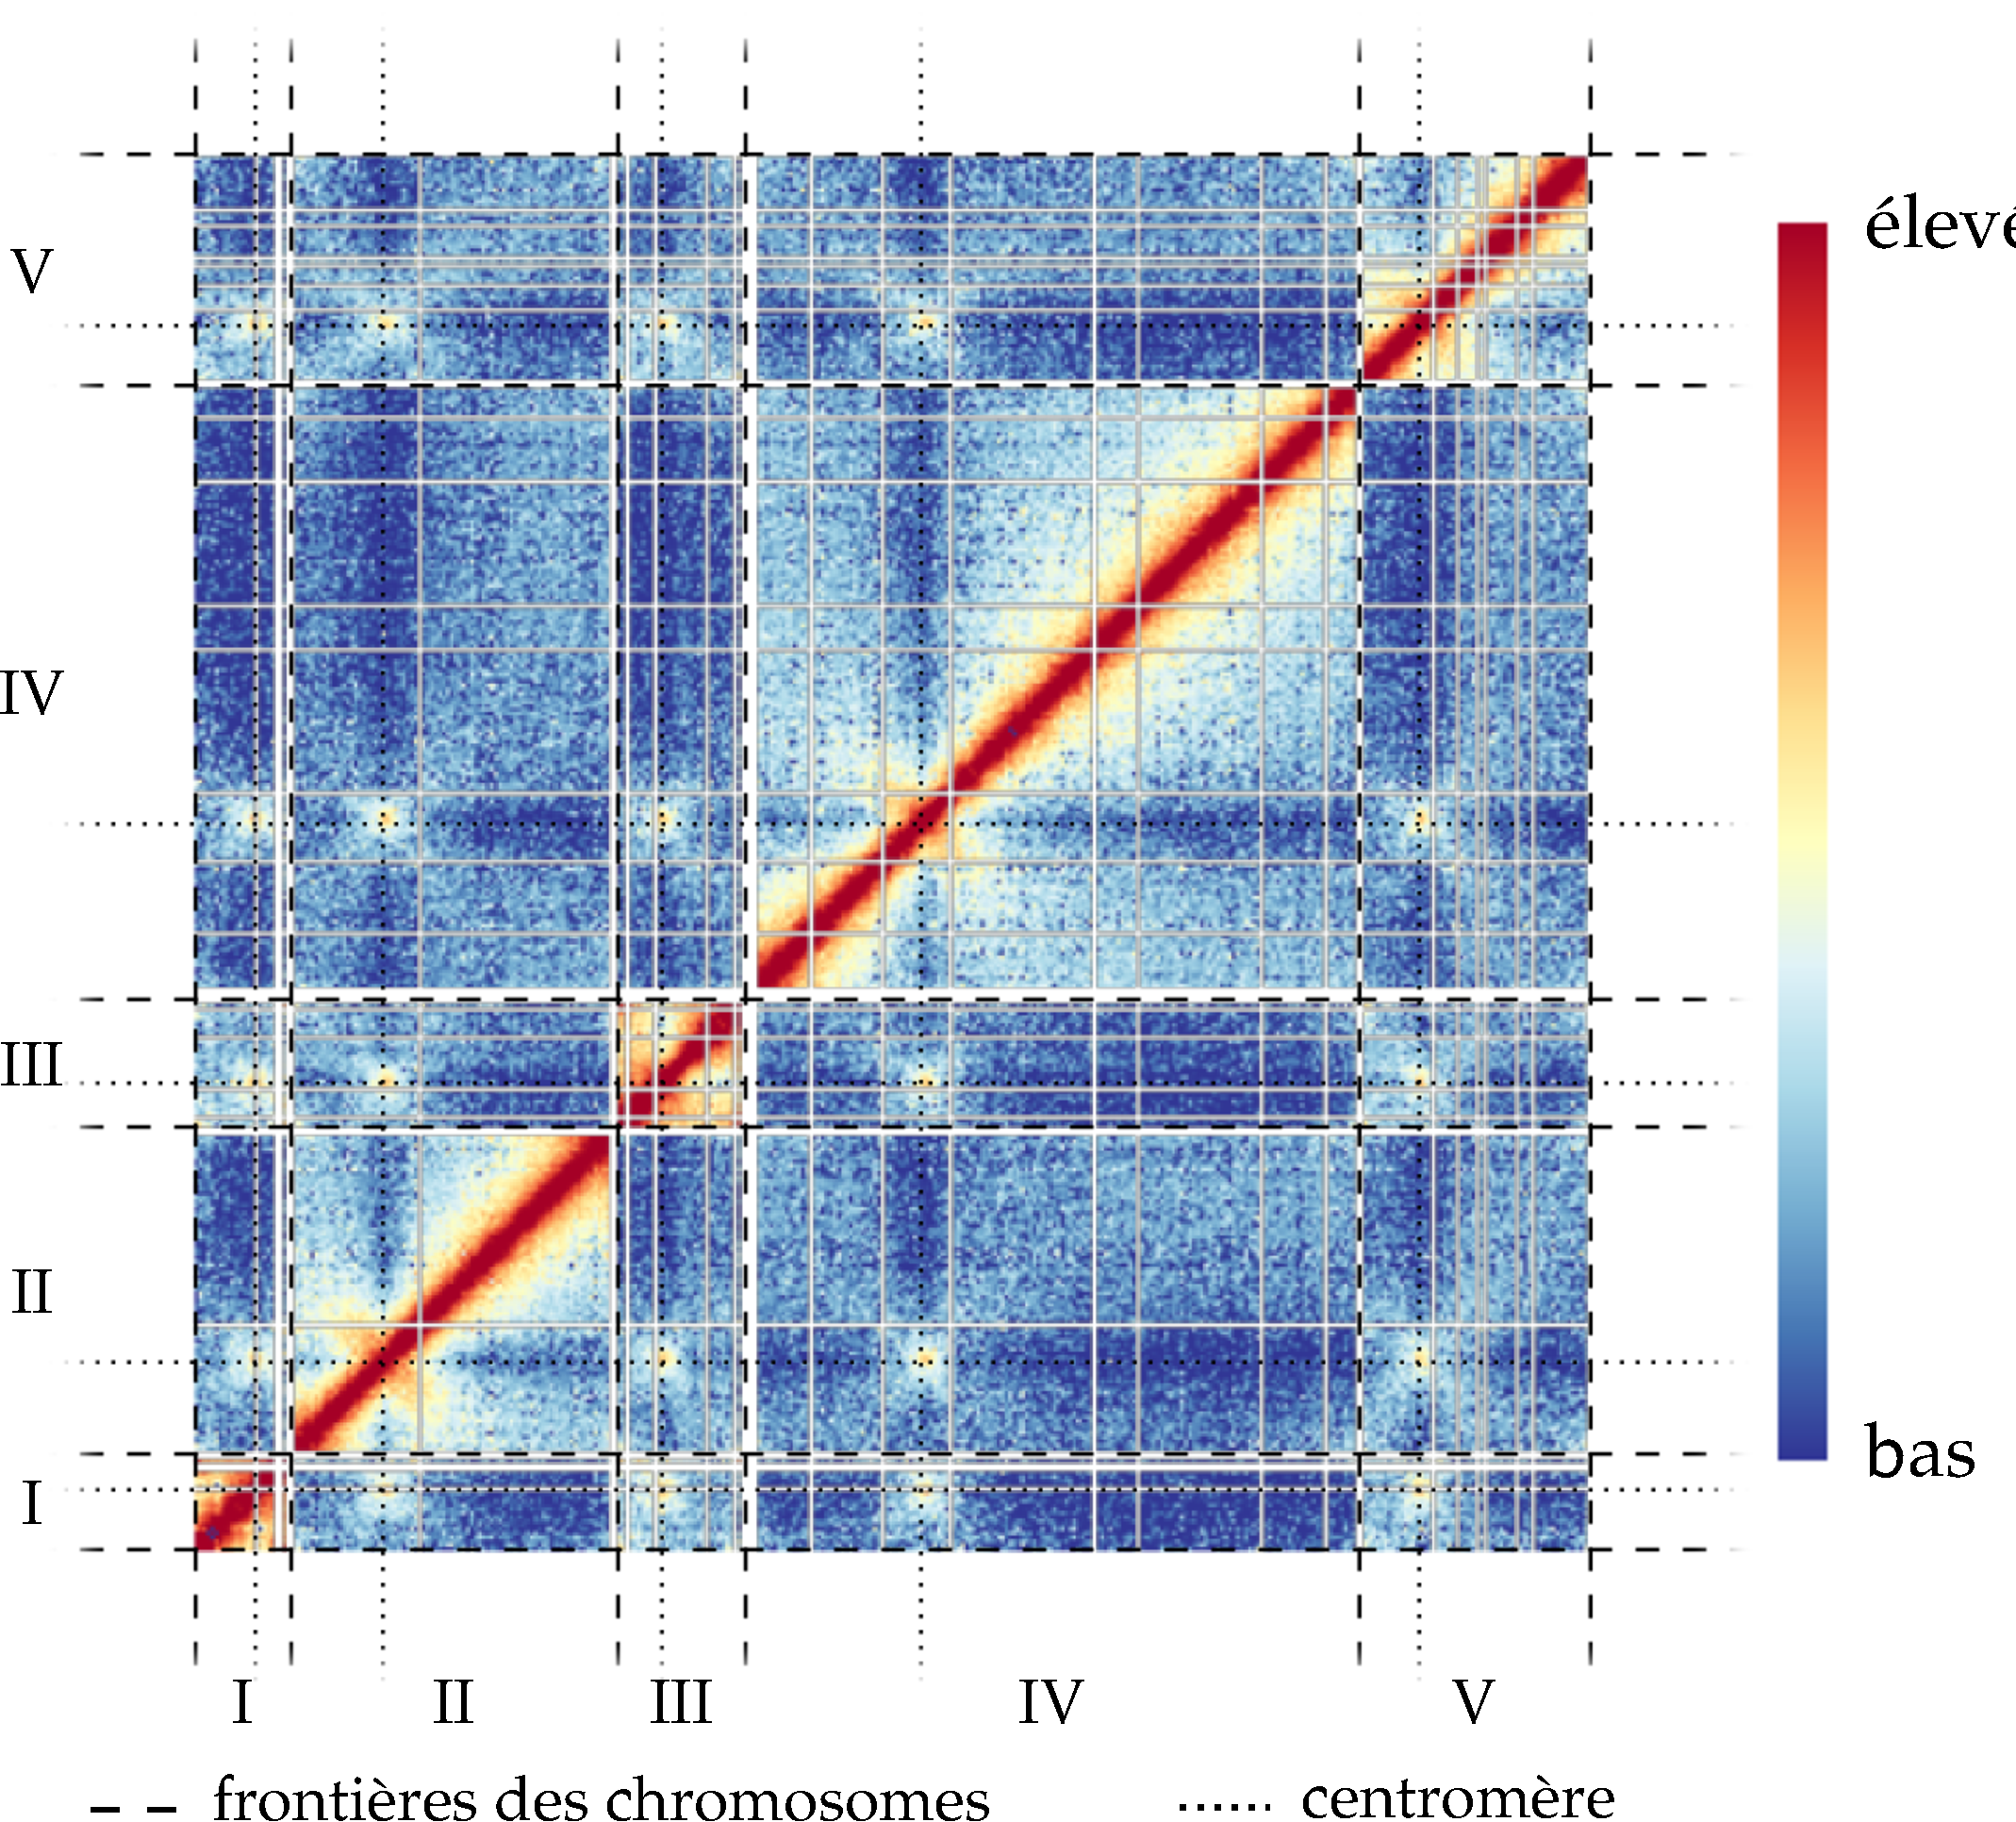
\includegraphics[width=0.45\textwidth]{figures/yeast_counts.pdf}
\end{center}}
\end{overlayarea}
\end{frame}

\section{Deconvolution of meta-genomic samples}
\begin{frame}
\Large{ \bf
Deconvolution of metagenomic samples}

\begin{flushright}
\vspace{1em}
\small

\textit{Joshua N. Burton*, Ivan Liachko*, Maitreya J. Dunham, Jay Shendure}
\end{flushright}
\end{frame}

\begin{frame}
\frametitle{Hi-C for metagenomic deconvolution}
\begin{center}
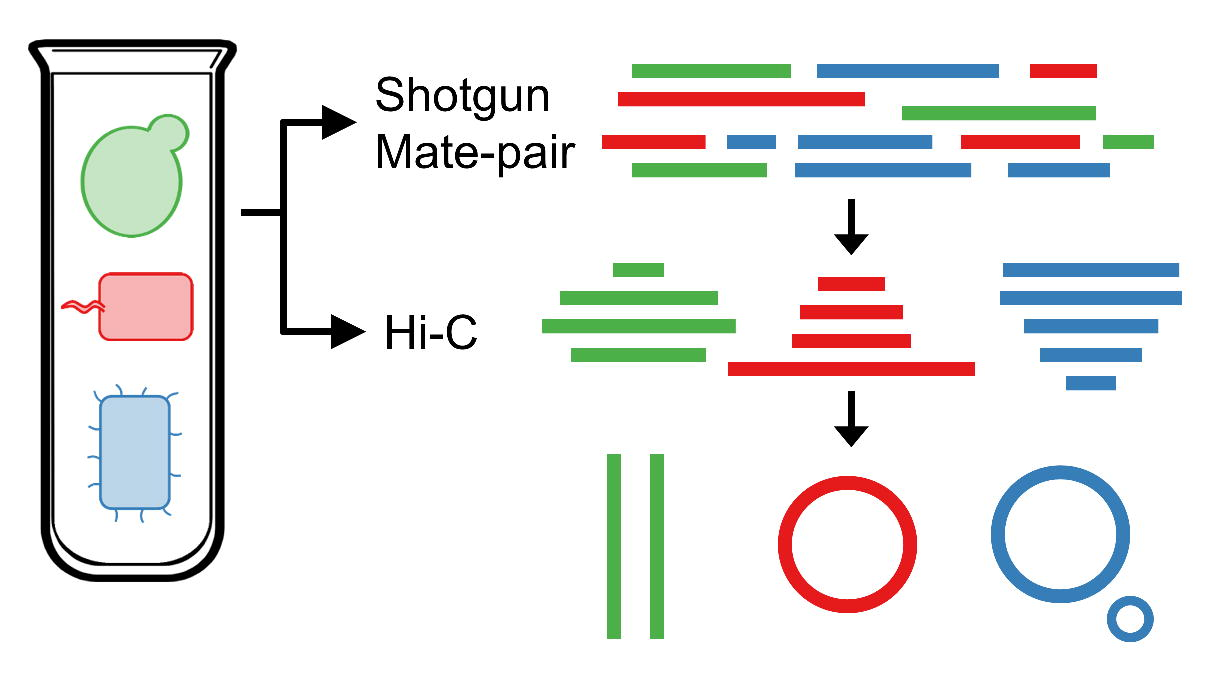
\includegraphics[width=0.75\linewidth]{figures/metagenomic_deconvolution.png}
\end{center}
\end{frame}


\begin{frame}
\frametitle{Hi-C for metagenomic deconvolution}
\begin{itemize}[label={$\bullet$}]
\item Assemble contigs using traditional shotgun sequencing;
\item Map the Hi-C reads to the contigs;
\item Cluster contigs with one another;
\item Find the permutation that orders the rows and columns in a statisfactory
manner.
\end{itemize}
\end{frame}

\begin{frame}
\frametitle{Clustering contigs}

\begin{itemize}[label={$\bullet$}]
\item Jarvis-Patrick nearest-neighbor clustering algorithm;
\item This nearest-neighbor approach accounts for differences in densities
between species;
\end{itemize}
\end{frame}

\begin{frame}
\frametitle{Genome scaffolding using Lachesis}
\begin{columns}
\begin{column}{0.59\linewidth}
\begin{itemize}[label={$\bullet$}]
\item Builds a graph where nodes are contings, and edges are inversily
proportional to contact count weight;
\item Minimum spanning tree applied on this graph to order contigs;
\item Exact positions of links to predict the relative orientation of contigs.
\end{itemize}
\end{column}
\begin{column}{0.49\linewidth}
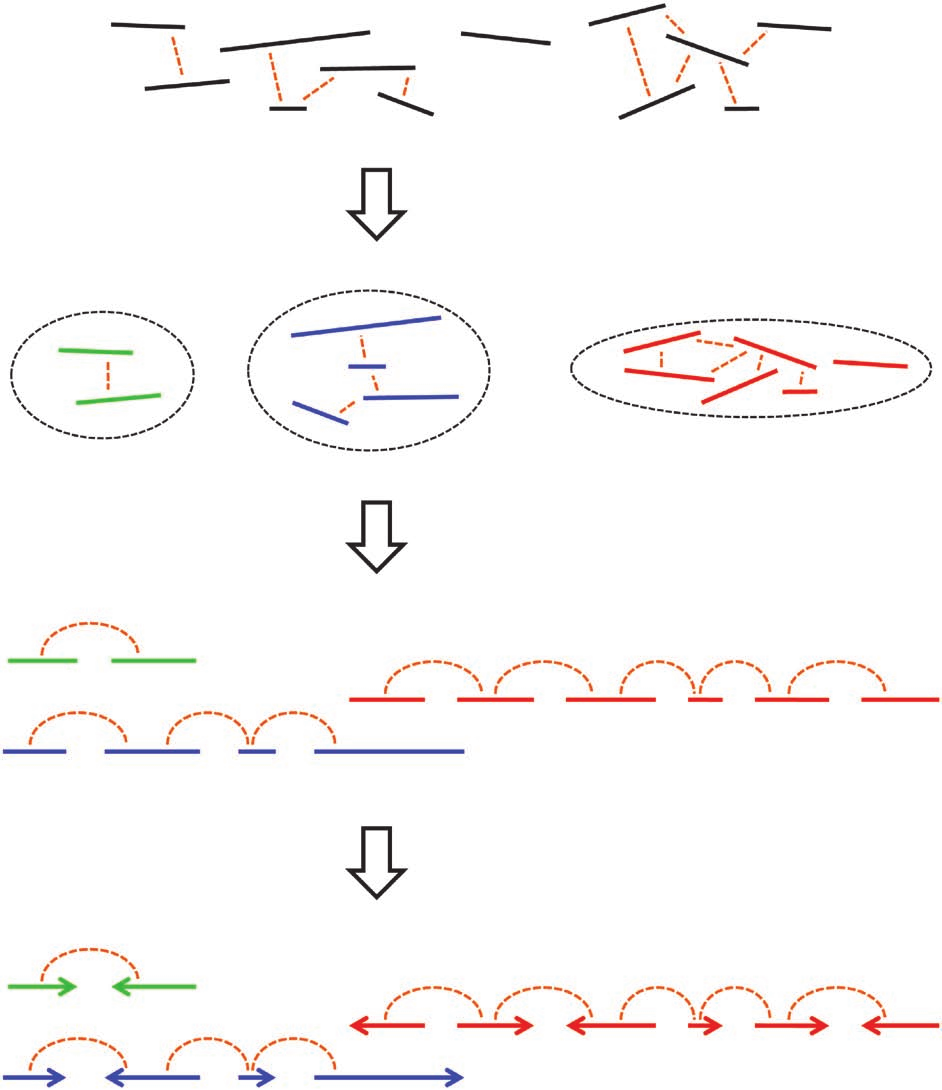
\includegraphics[width=\linewidth]{figures/lachesis_scaffolding.png}
\end{column}
\end{columns}
\end{frame}

\section{Accurate identification of centromere location in yeasts using Hi-C}
\begin{frame}
\Large{ \bf
Accurate identification of centromere locations in yeasts using Hi-C.}

\begin{flushright}
\vspace{1em}
\small

\textit{joint work with  Ivan Liachko, Josh Burton, \\
Ferhat Ay, Jay Shendure, Maitreya Dunham, \\ Jean-Philippe Vert and William S.
Noble 
}
\end{flushright}

\end{frame}

% 1. Introduction of the yeasts genome architecture -> Rabl conformation
\begin{frame}
\frametitle{Yeasts are widely studied, widely used organisms}
\only<1>{

\includegraphics[width=0.9\linewidth]{figures/plasmids_without_centromeres_1.eps}
}
\only<2>{
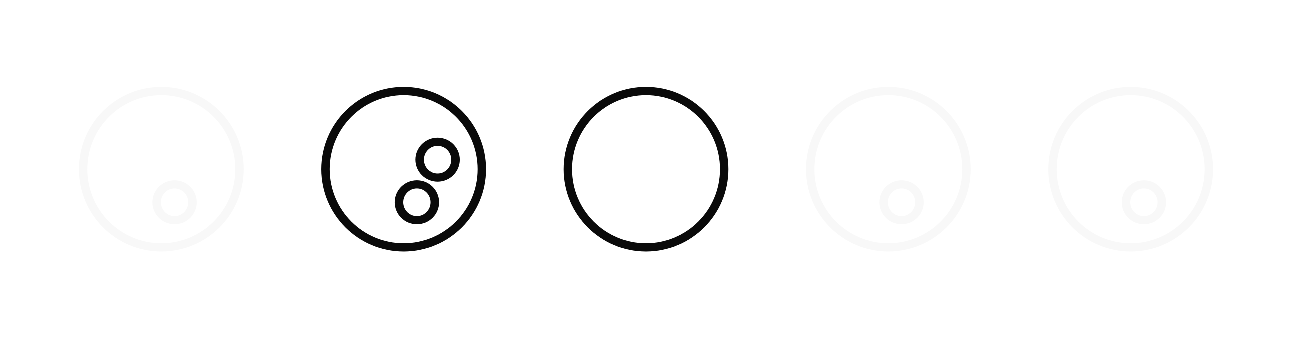
\includegraphics[width=0.9\linewidth]{figures/plasmids_without_centromeres_2.eps}
}
\only<3>{
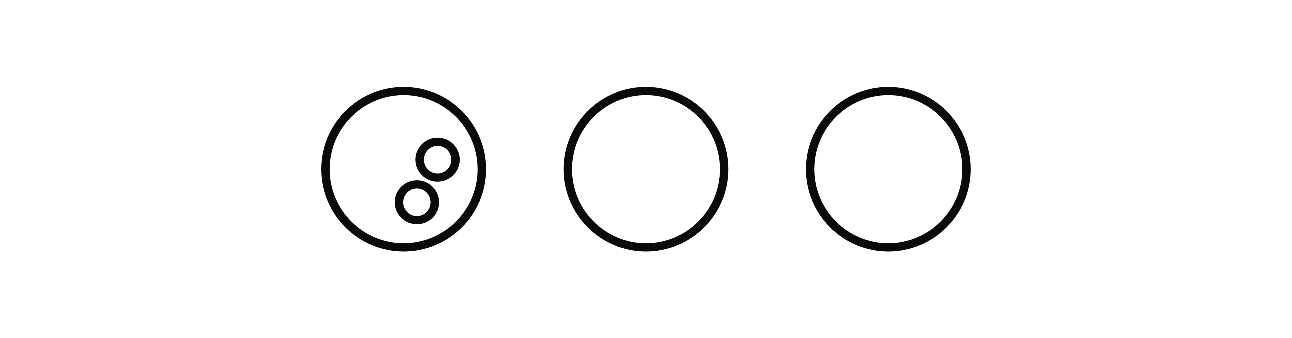
\includegraphics[width=0.9\linewidth]{figures/plasmids_without_centromeres_3.eps}
}
\only<4>{
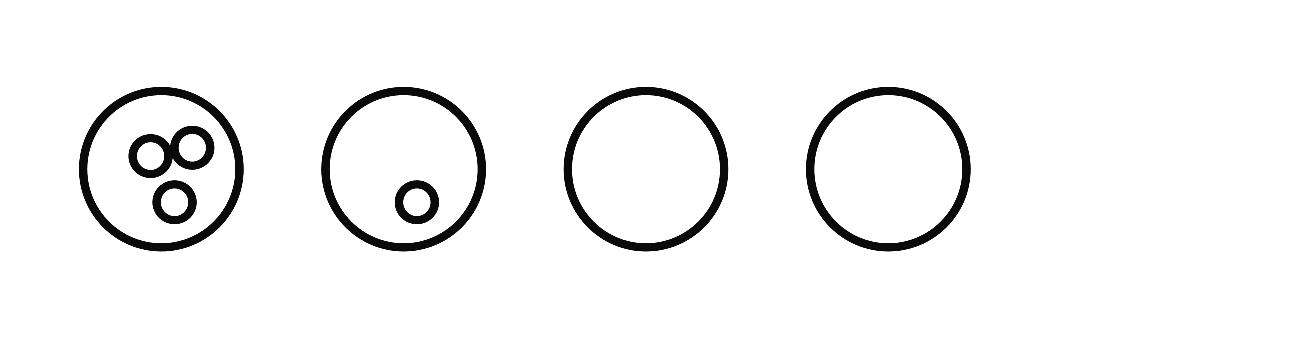
\includegraphics[width=0.9\linewidth]{figures/plasmids_without_centromeres_4.eps}
}
\only<5>{
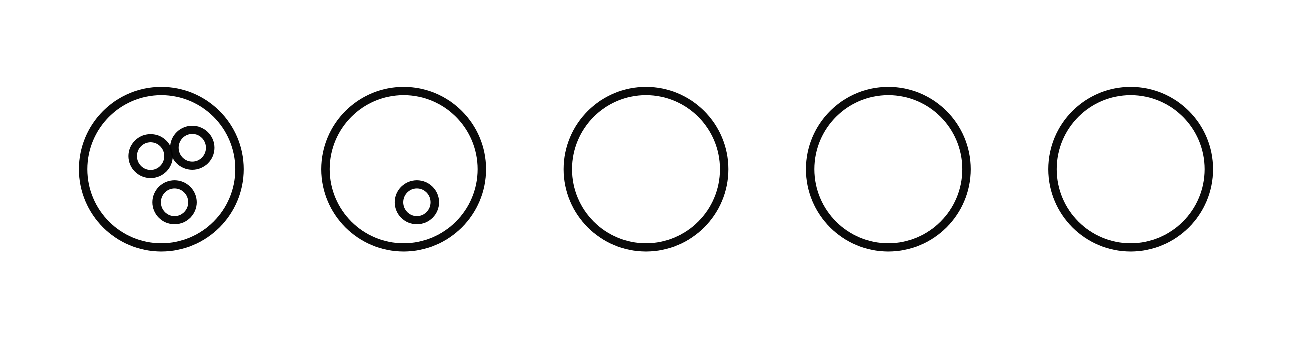
\includegraphics[width=0.9\linewidth]{figures/plasmids_without_centromeres_5.eps}
}
\only<6>{
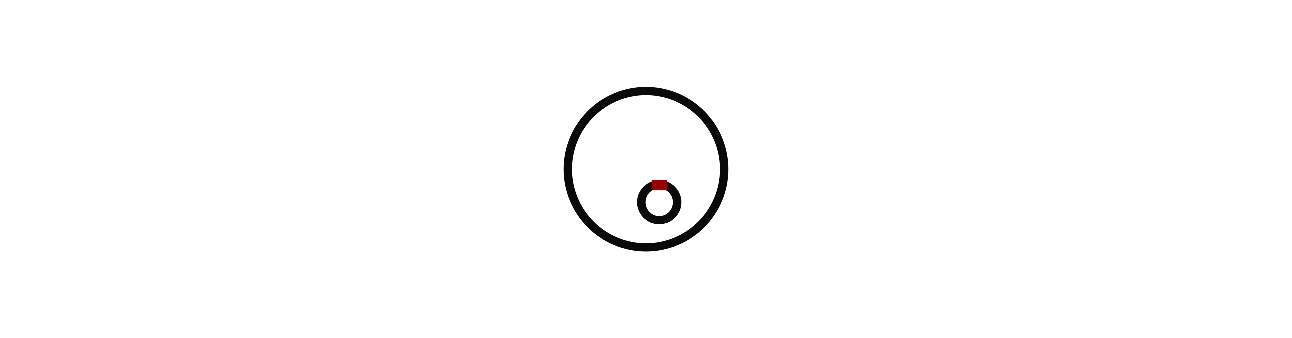
\includegraphics[width=0.9\linewidth]{figures/plasmids_with_centromeres_1.eps}
}
\only<7>{
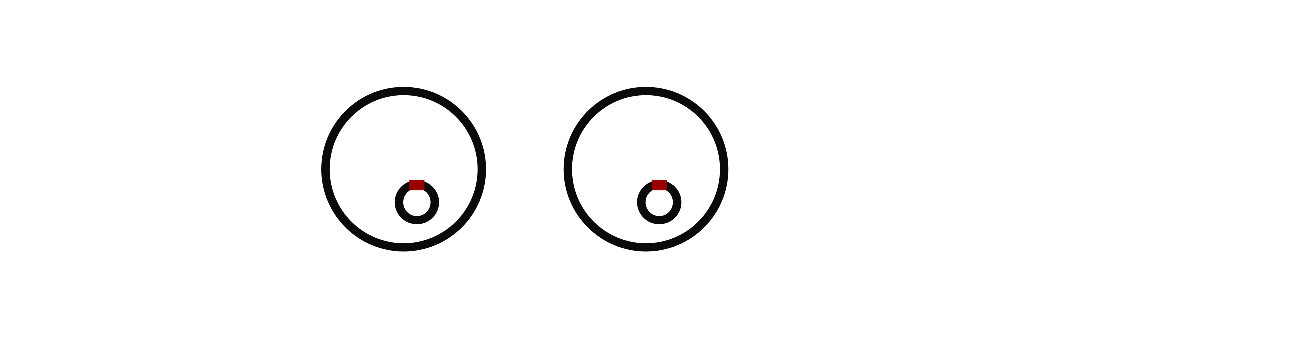
\includegraphics[width=0.9\linewidth]{figures/plasmids_with_centromeres_2.eps}
}
\only<8>{
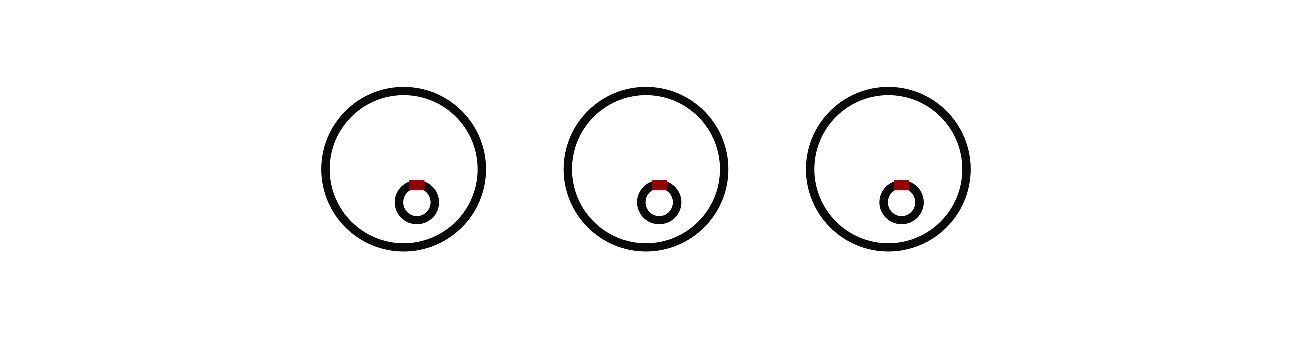
\includegraphics[width=0.9\linewidth]{figures/plasmids_with_centromeres_3.eps}
}
\only<9>{
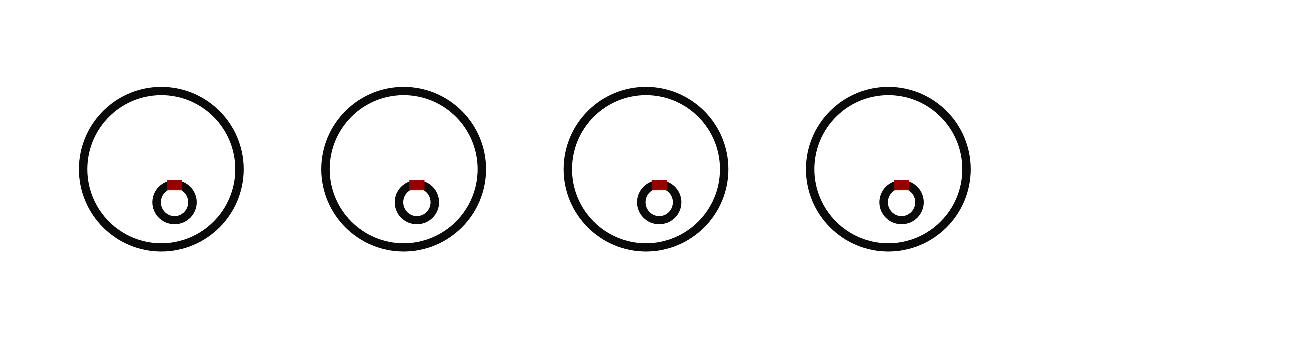
\includegraphics[width=0.9\linewidth]{figures/plasmids_with_centromeres_4.eps}
}
\only<10>{
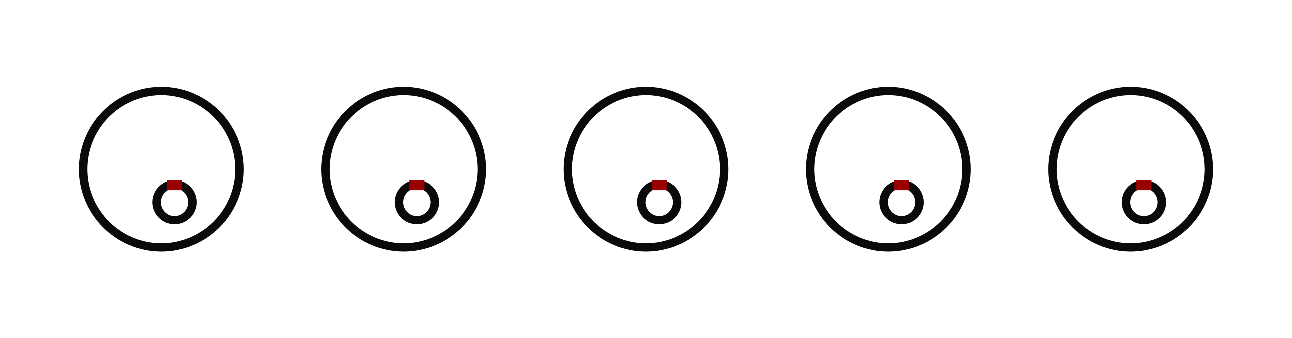
\includegraphics[width=0.9\linewidth]{figures/plasmids_with_centromeres_5.eps}
}

{\color{Blue} \textbf{Motivation}}
\begin{itemize}
\item Yeasts are crucial organisms in biotechnology applications.
\item Centromeres allow proper segregation of chromosomes.
\end{itemize}

\vspace{1em}
{\color{Blue} \textbf{Goal}} Develop a robust and accurate method to detect
centromere locations in yeasts.

\vspace{1em}
{\color{Blue} \textbf{Idea}} Leverage the yeasts' genome architecture (where
centromeres colocalize) and Hi-C
data to detect centromere locations.
\end{frame}

% 2. Motivation
\begin{frame}
\frametitle{Yeasts' centromeres colocalize in the nucleus}
\begin{figure}
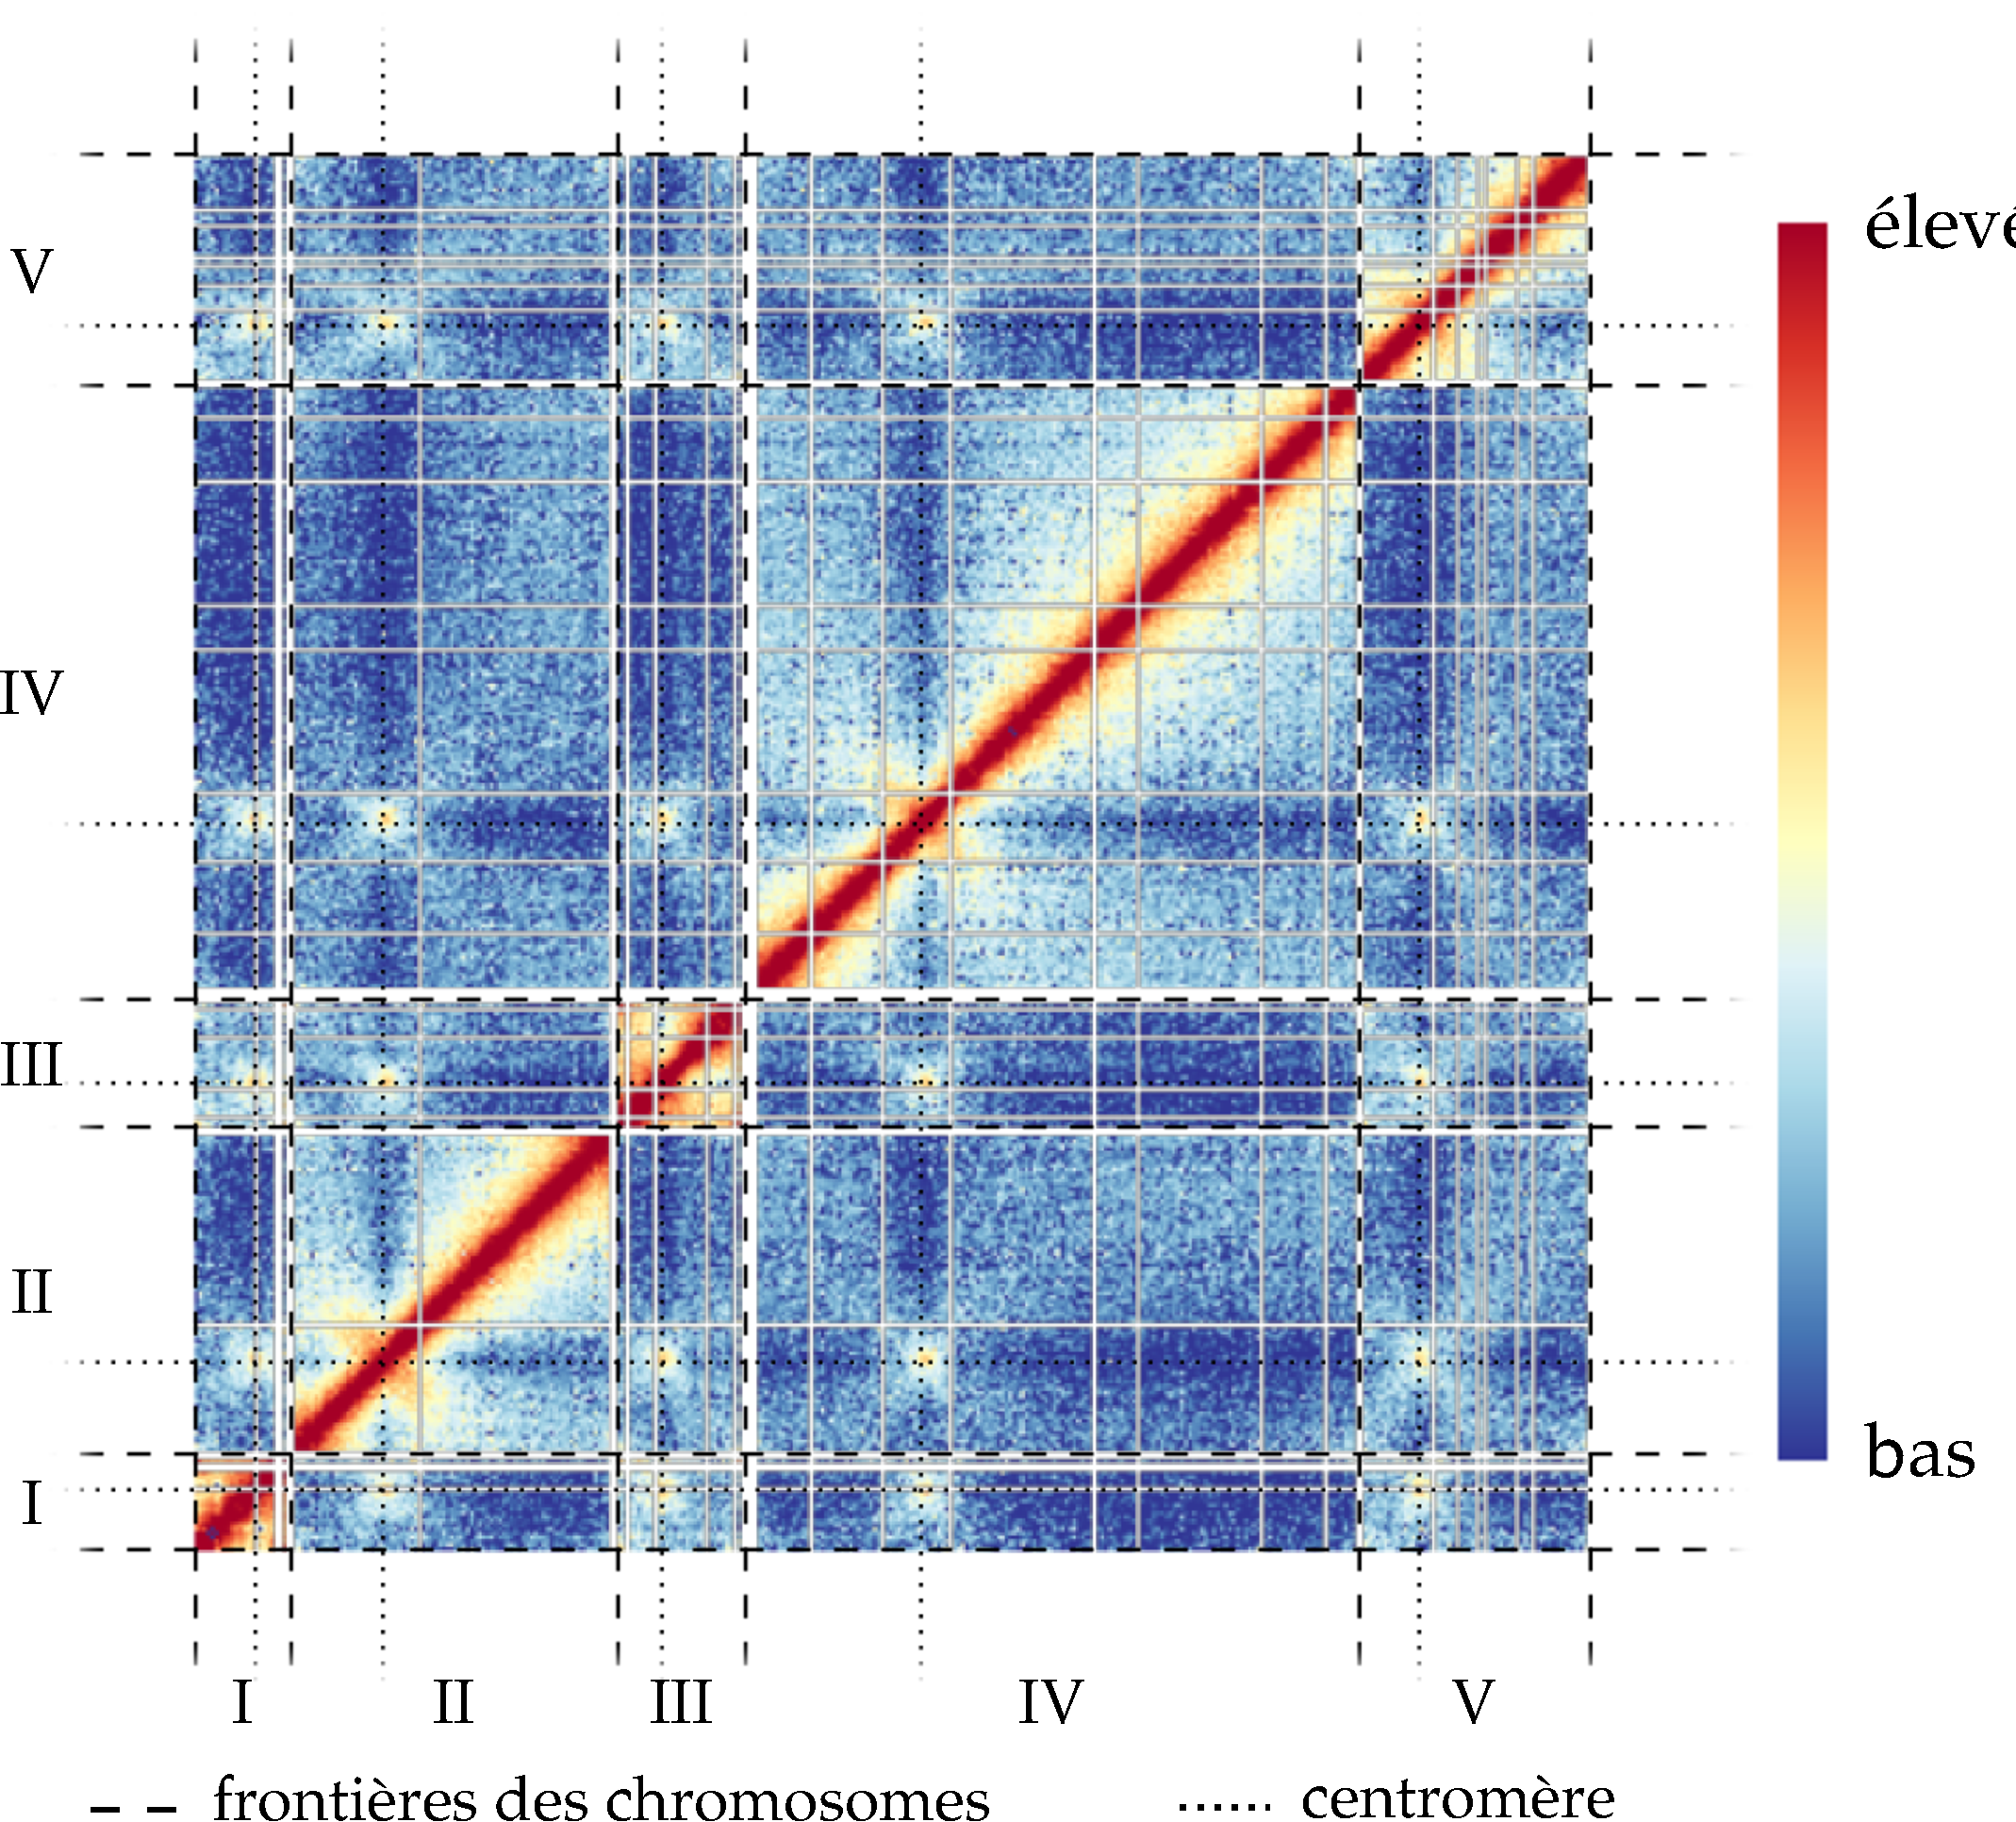
\includegraphics[width=0.52\textwidth]{figures/yeast_counts.pdf}
\caption{Contact counts for the first 5 chromosomes of \textit{S. cerevisiae}}
\end{figure}
\end{frame}

\begin{frame}
\frametitle{Centurion in brief}
\begin{figure}
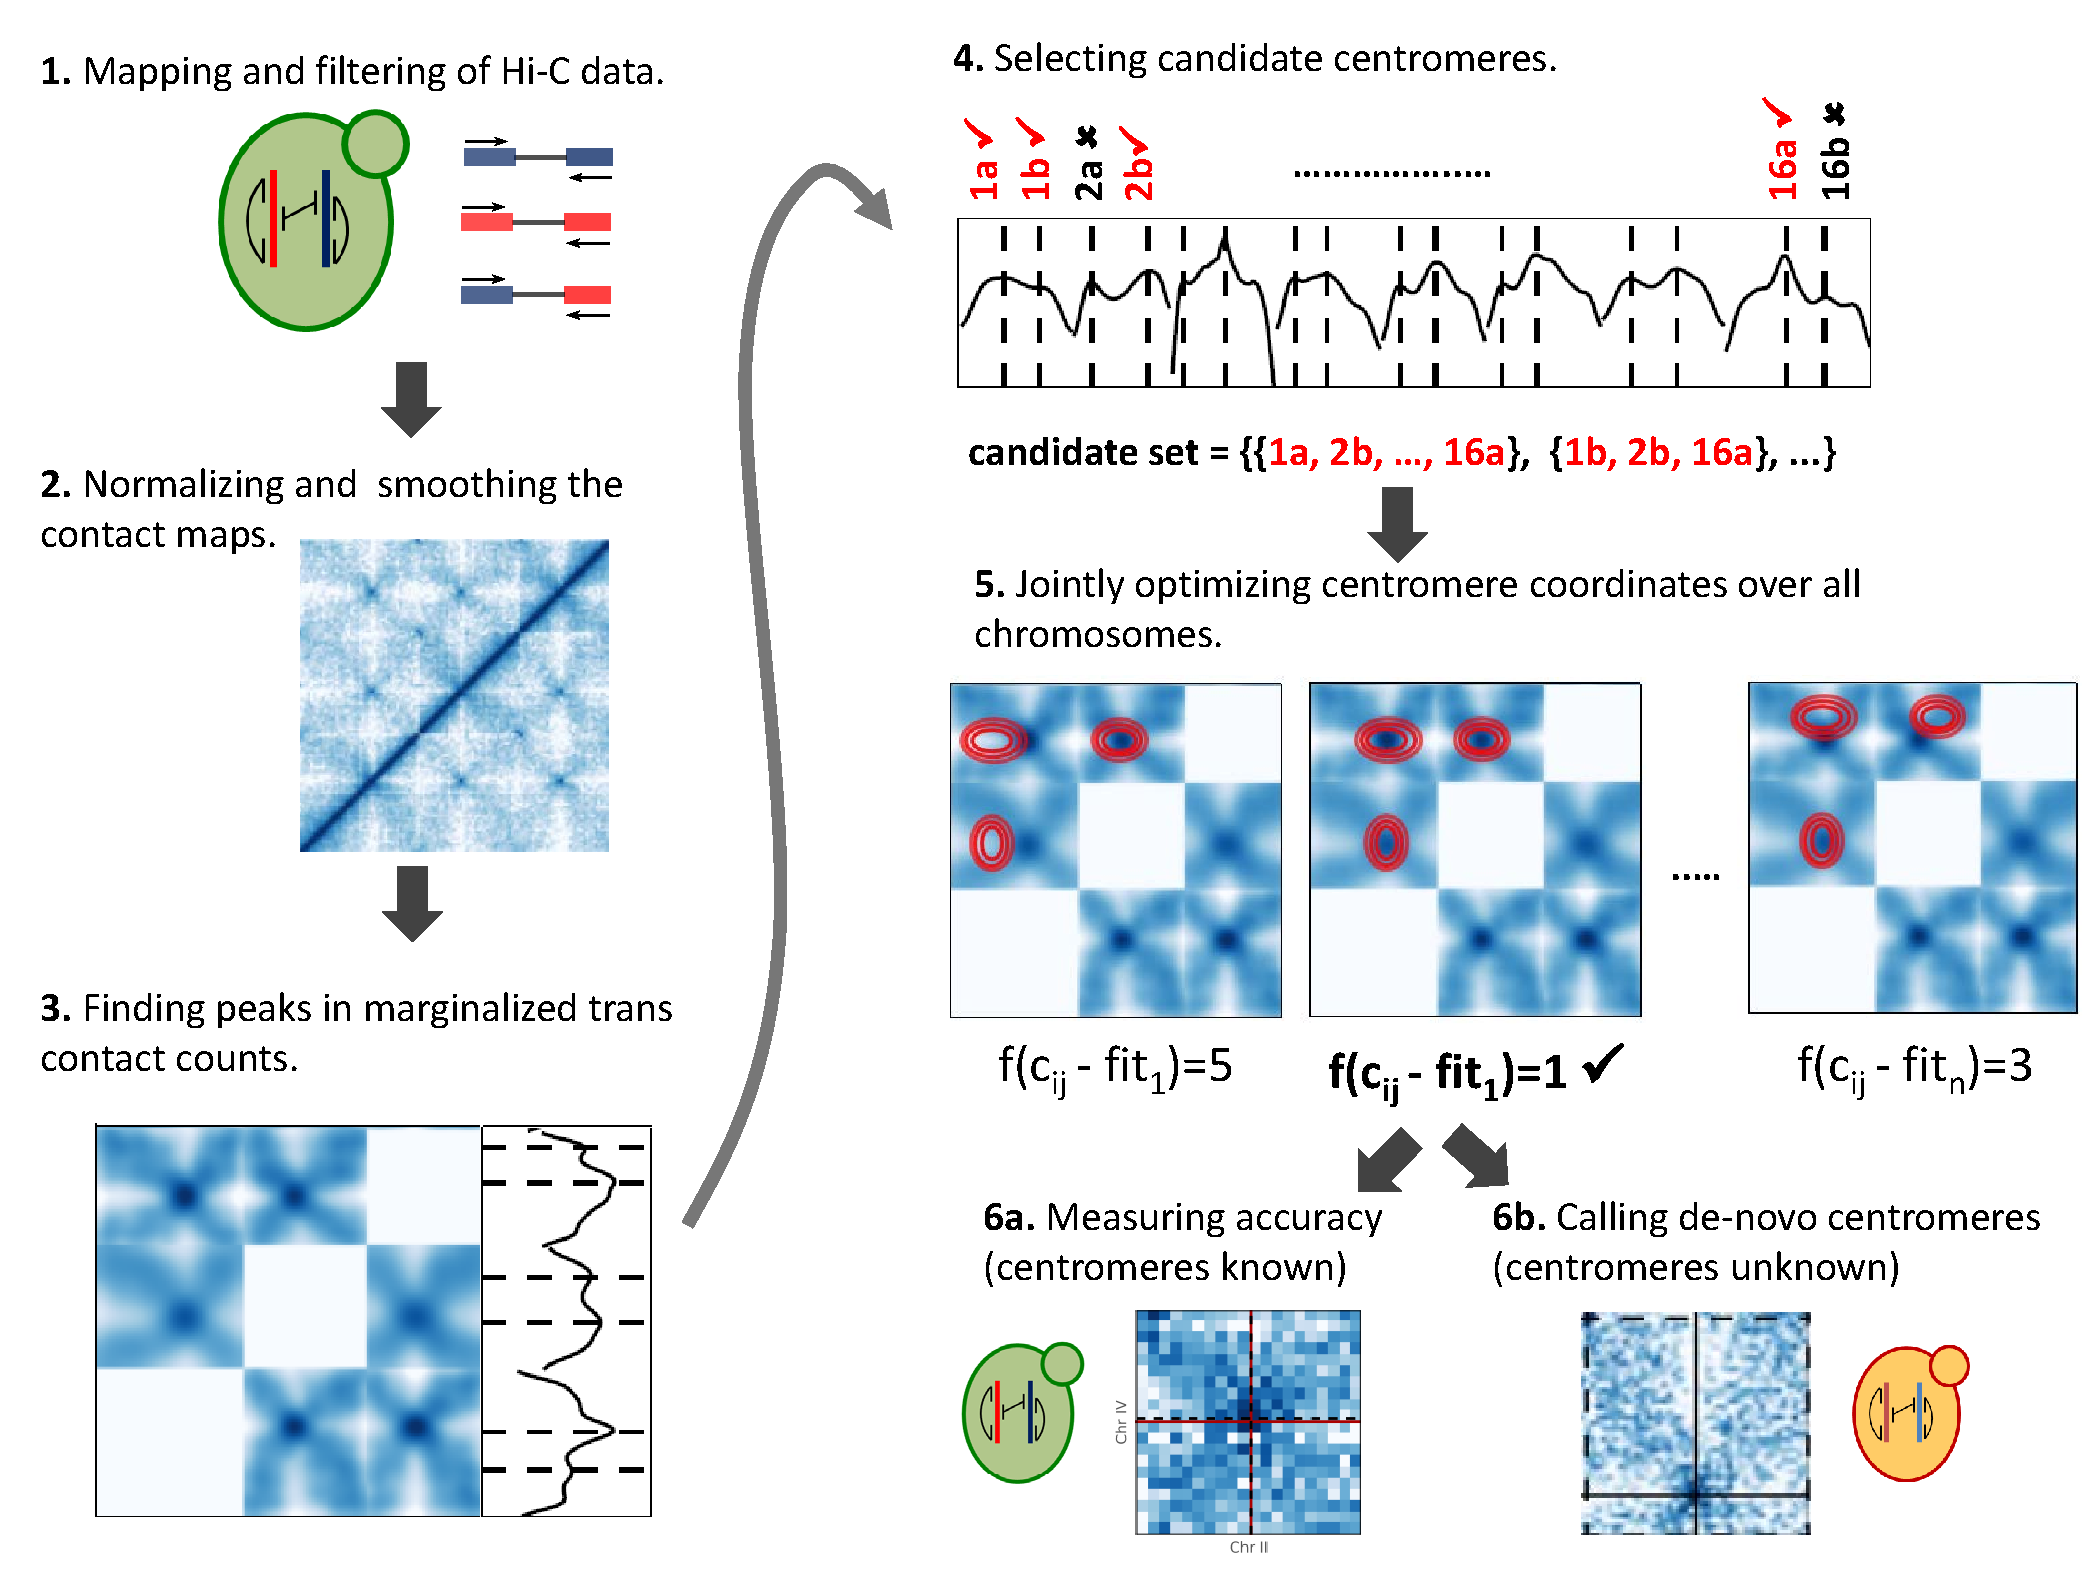
\includegraphics[width=0.85\textwidth]{figures/centurion_brief.pdf}
\end{figure}
\end{frame}

% 3. Idea
\begin{frame}
\frametitle{Contact enrichment as a Gaussian function}
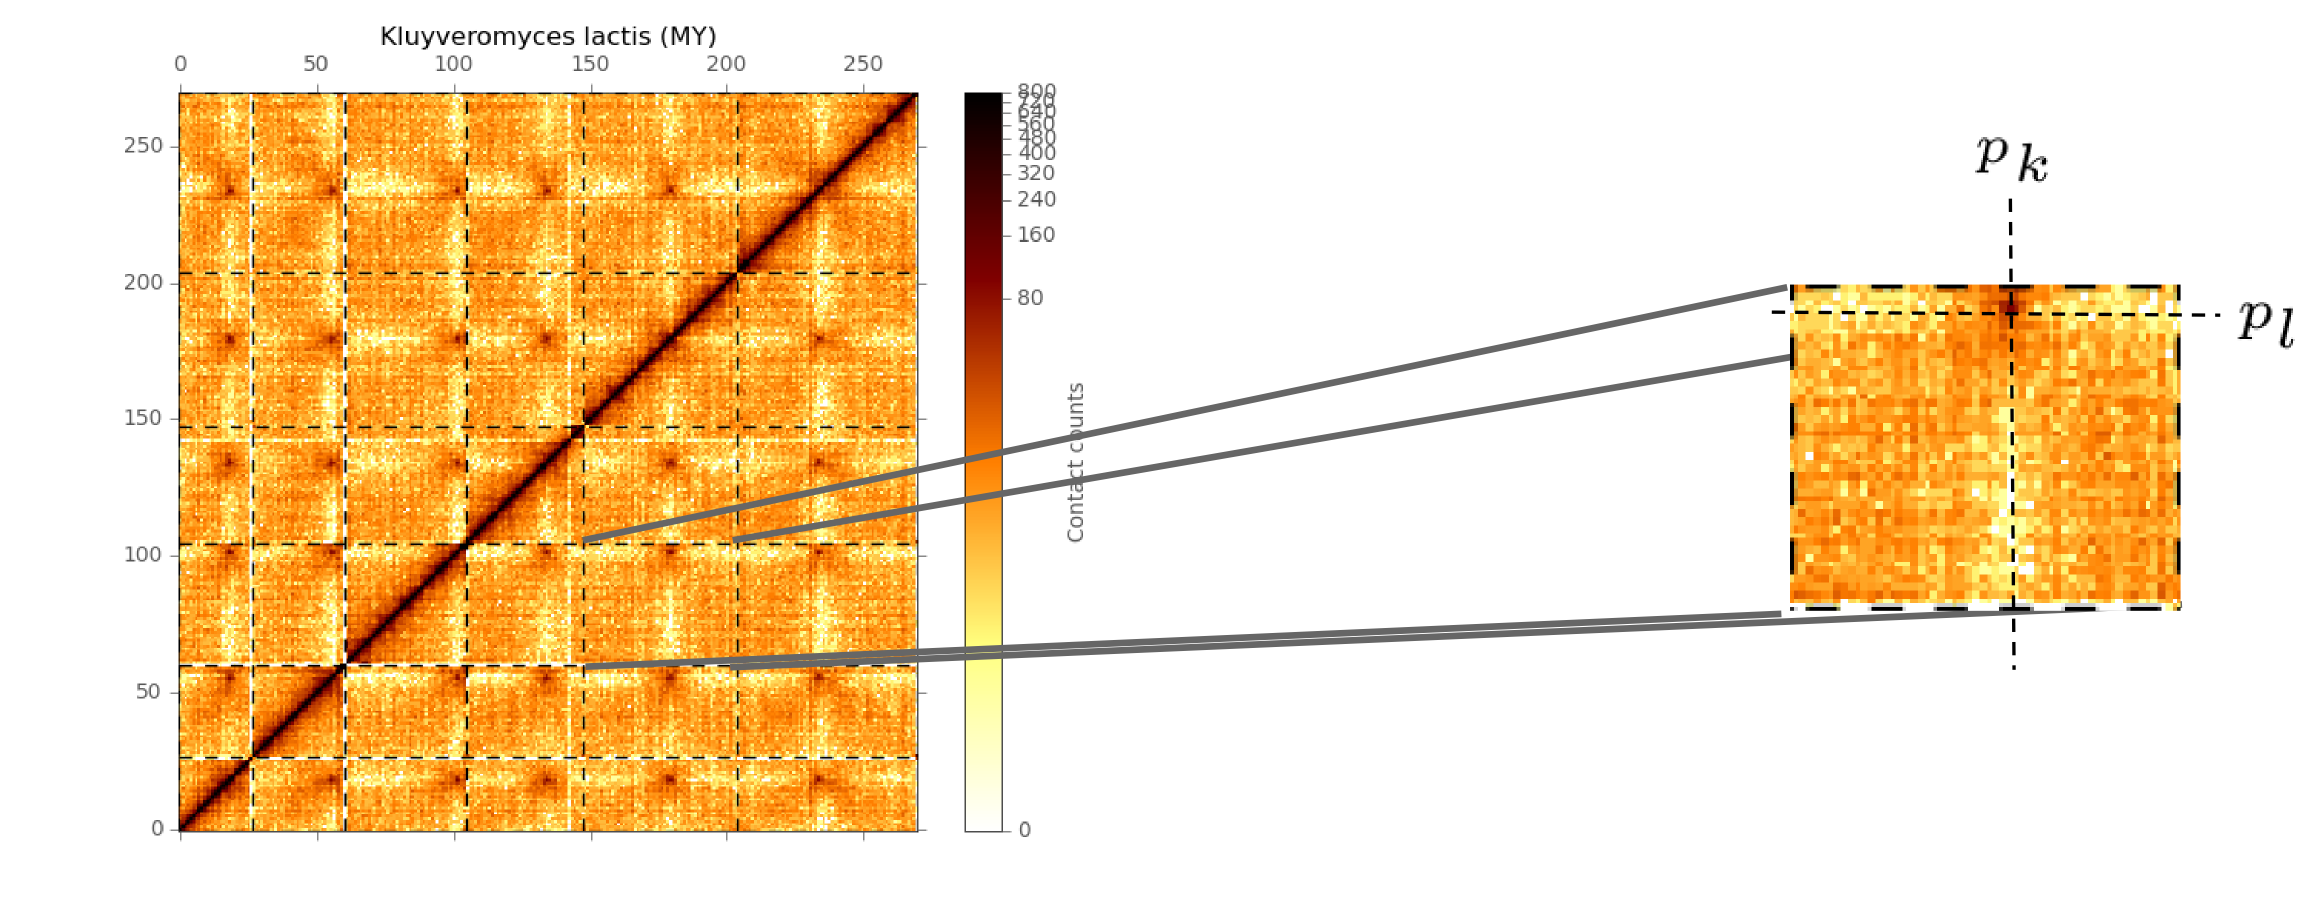
\includegraphics[width=\linewidth]{figures/centurion_idea.png}
\begin{flushright}
$a\exp \left(- \frac{(x_i -
p_k)^2 + (x_j - p_l)^2)}{2\sigma^2}\right)$
\end{flushright}
\end{frame}

% 4. Optimization problem
\begin{frame}
\frametitle{Centromere detection as an optimization problem}

\begin{equation*}
\renewcommand{\arraystretch}{2}
\begin{array}{ccll}
\underset{\textbf{P}, a, \sigma, b}{\text{minimize}} & &
\sum_{(i,j)\in\mathcal{D}} \left[ c_{ij} - a\exp \left(- \frac{(x_i -
p_{B(i)})^2 + (x_j - p_{B(j)})^2)}{2\sigma^2}\right) - b \right]^2\,. \\
\text{subject to} & & p_i\quad\text{belongs to chromosome }i
\end{array}
\end{equation*}

where
\begin{itemize}[label={$\bullet$}]
\item $B(i)$ is a mapping between locus $i$ and its chromosome.
\item $p_{B(i)}$ corresponds to the centromere candidate of locus $i$'s
chromosome.
\end{itemize}
\end{frame}

\begin{frame}
\frametitle{Initializing the optimization problem}

{\color{Blue} \bf Problems}
\begin{itemize}[label={$\bullet$}]
\item The objective function is non convex.
\item Other DNA regions colocolize and highly interact with one another.
\end{itemize}

\vspace{1em}
{\color{Blue} \bf Solutions}
\begin{itemize}[label={$\bullet$}]
\item Use the inter chromosomal contact counts enrichments to identify
potential candidates (typically two per chromosomes).
\item Initialize the optimization with all possible combinations.
\end{itemize}

\end{frame}

% 5. Initialization
% 6. Results
\begin{frame}
\frametitle{Centromeres' call on \textit{S. cerevisiae}}
\begin{figure}
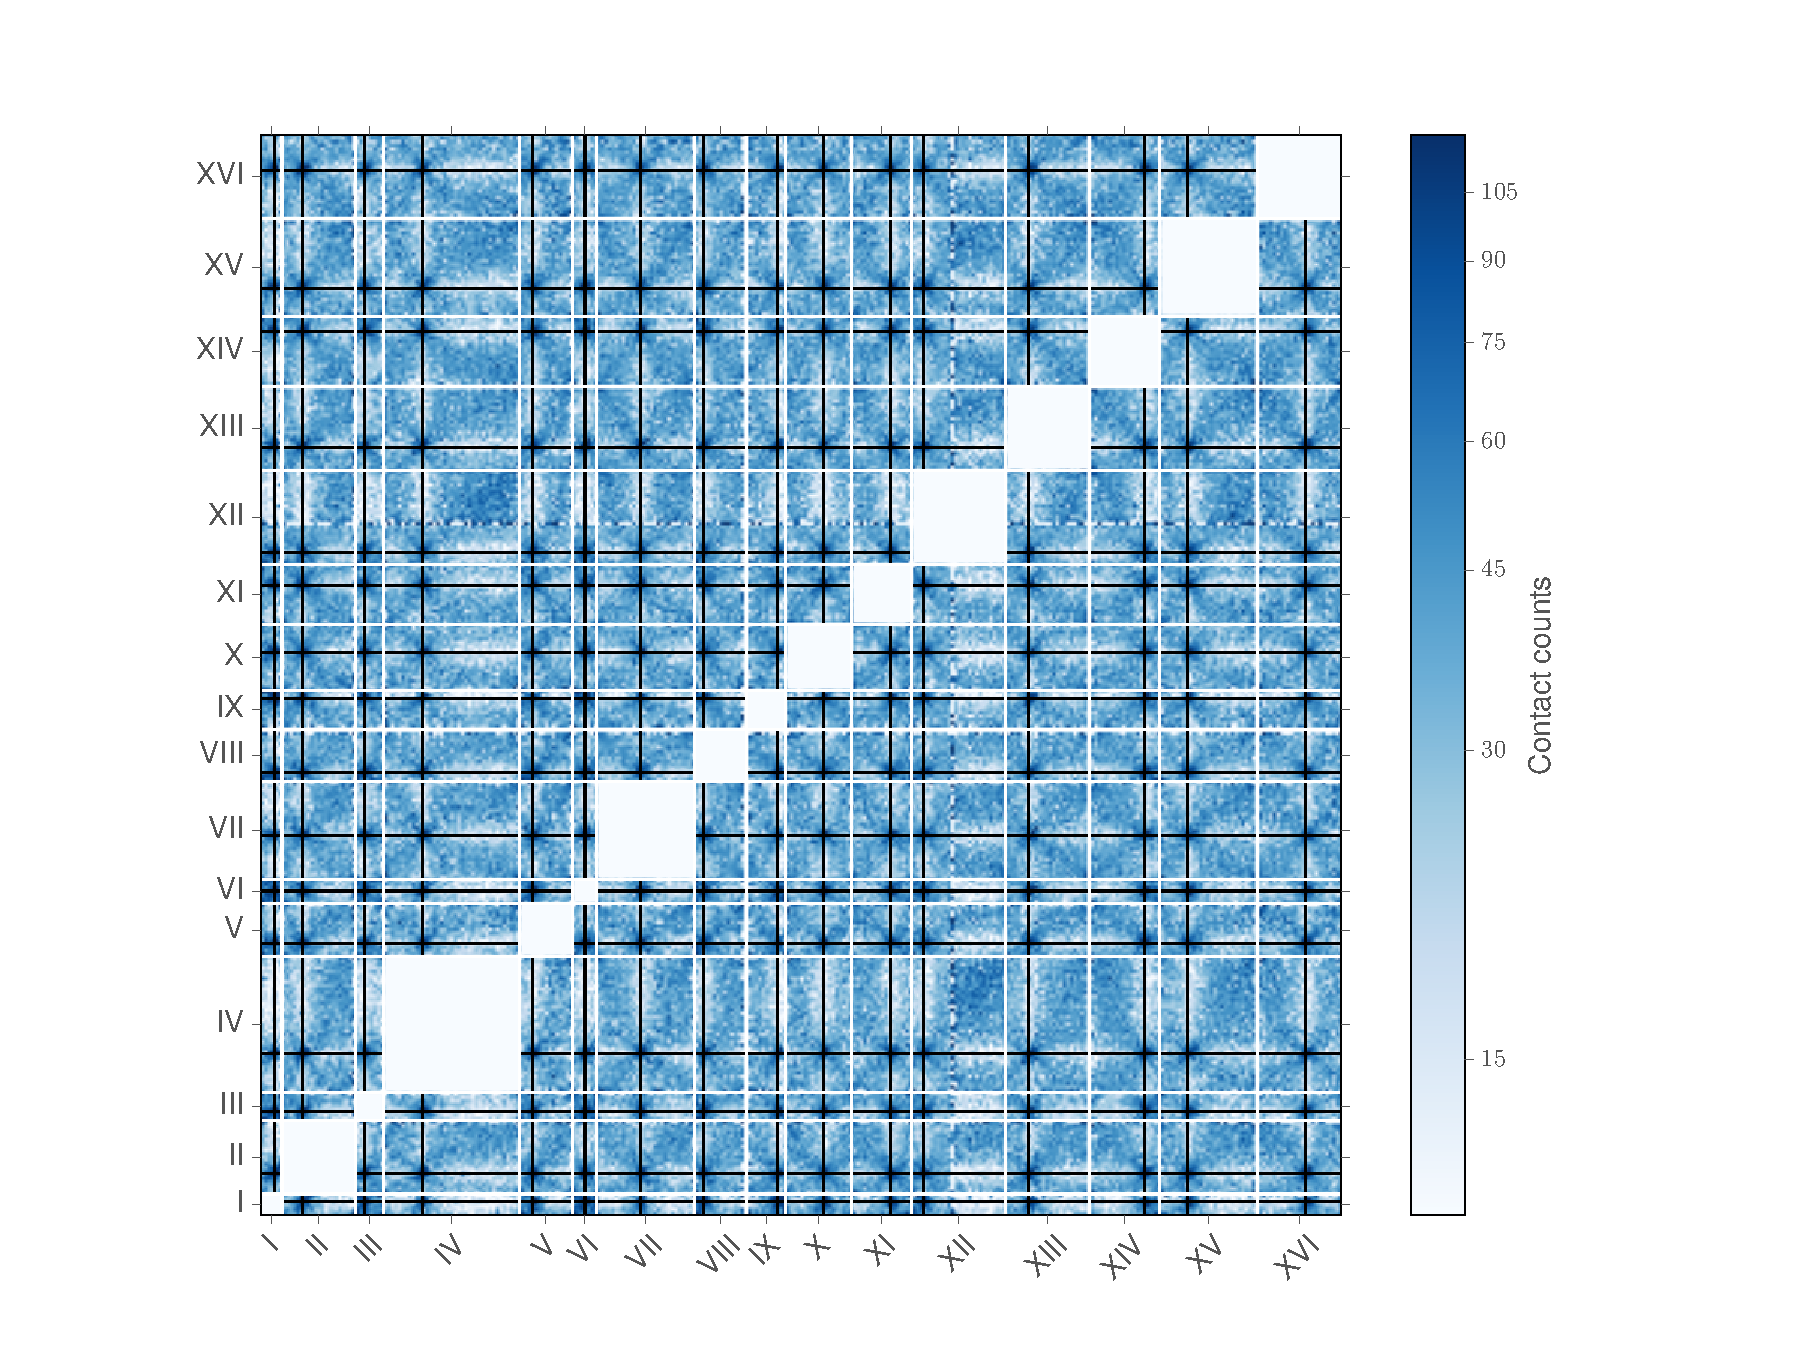
\includegraphics[width=0.9\linewidth]{figures/2_whole_genome_SC.pdf}
\end{figure}
\end{frame}


\begin{frame}
\frametitle{Centurion accurately predicts centromere locations}
\begin{figure}
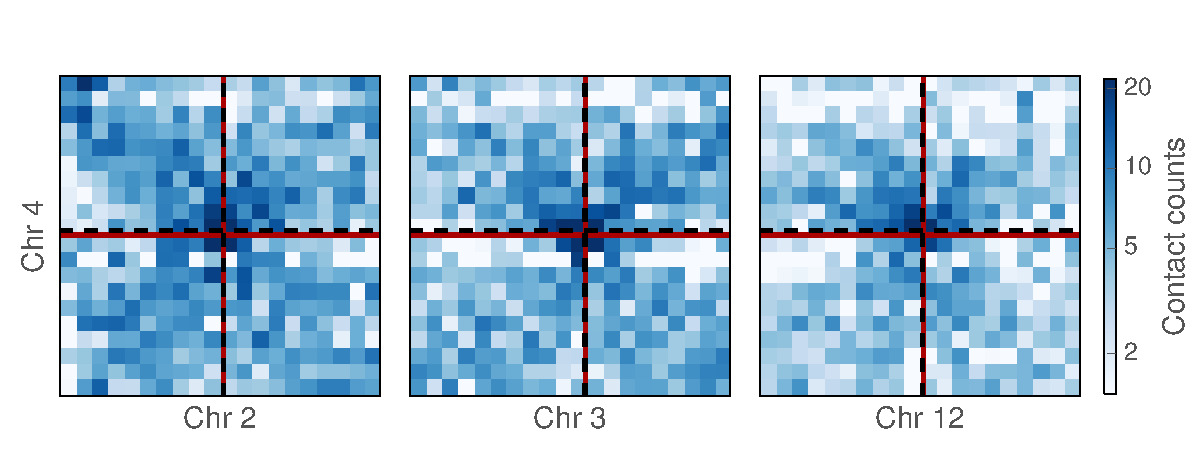
\includegraphics[width=0.9\linewidth]{figures/2_pf_zoomed_in.pdf}
\caption{Centromere calling on \textit{P. falciparum}}
\end{figure}
\end{frame}

\begin{frame}
\frametitle{The \citet{marie-nelly:filling} method for centromere detection}

\citet{marie-nelly:filling} propose a two-step method:
\vspace{2em}

\begin{columns}
\begin{column}{0.5\textwidth}
\textbf{1. Prelocalizing centromeres}
\end{column}
\begin{column}{0.5\textwidth}
\textbf{2. Refining the prediction}
\end{column}
\end{columns}

\begin{columns}
\centering
\begin{column}{0.5\textwidth}
\begin{center}
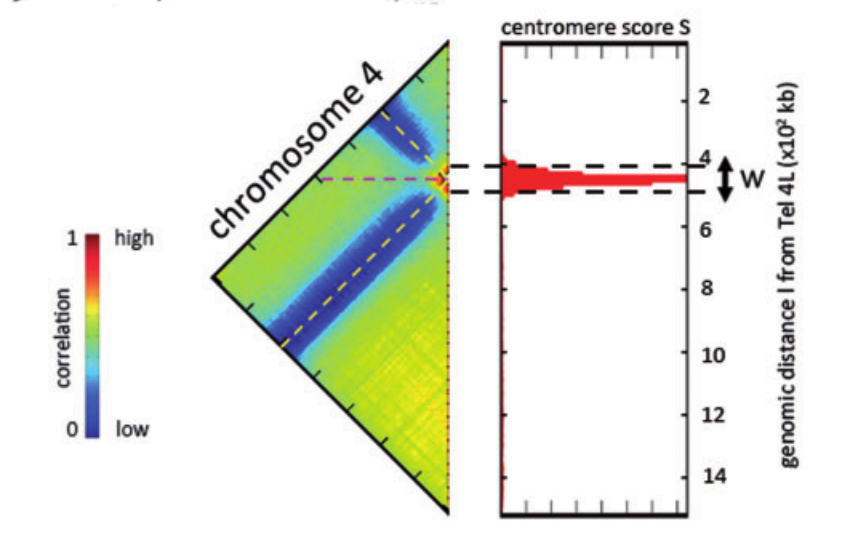
\includegraphics[width=0.75\textwidth]{figures/marie_nelly_prelocation.png}
\end{center}
\end{column}
\begin{column}{0.5\textwidth}
\begin{center}
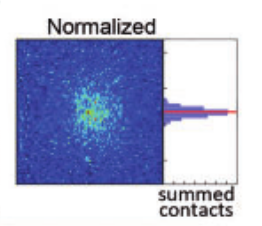
\includegraphics[width=0.5\textwidth]{figures/marie_nelly_step2.png}
\end{center}
\end{column}
\end{columns}

\end{frame}

\begin{frame}
\frametitle{Comparison of the objective functions}

\begin{figure}
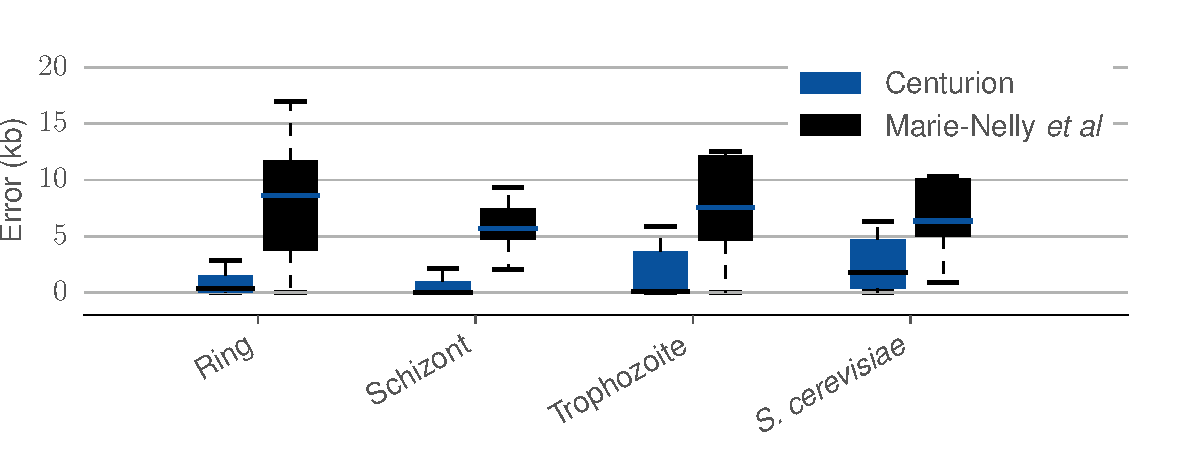
\includegraphics[width=0.9\linewidth]{figures/2_MN_vs_us_starting_gt_HR_40000.pdf}
\end{figure}
\end{frame}

\begin{frame}
\frametitle{De novo centromere calls on 6 yeast species}

\textit{K. wickerhamii}, \textit{P. pastoris}, \textit{S. paradoxus}, \textit{L.
waltii}, \textit{E. gossypii}, \textit{S. stipitis}

\begin{figure}
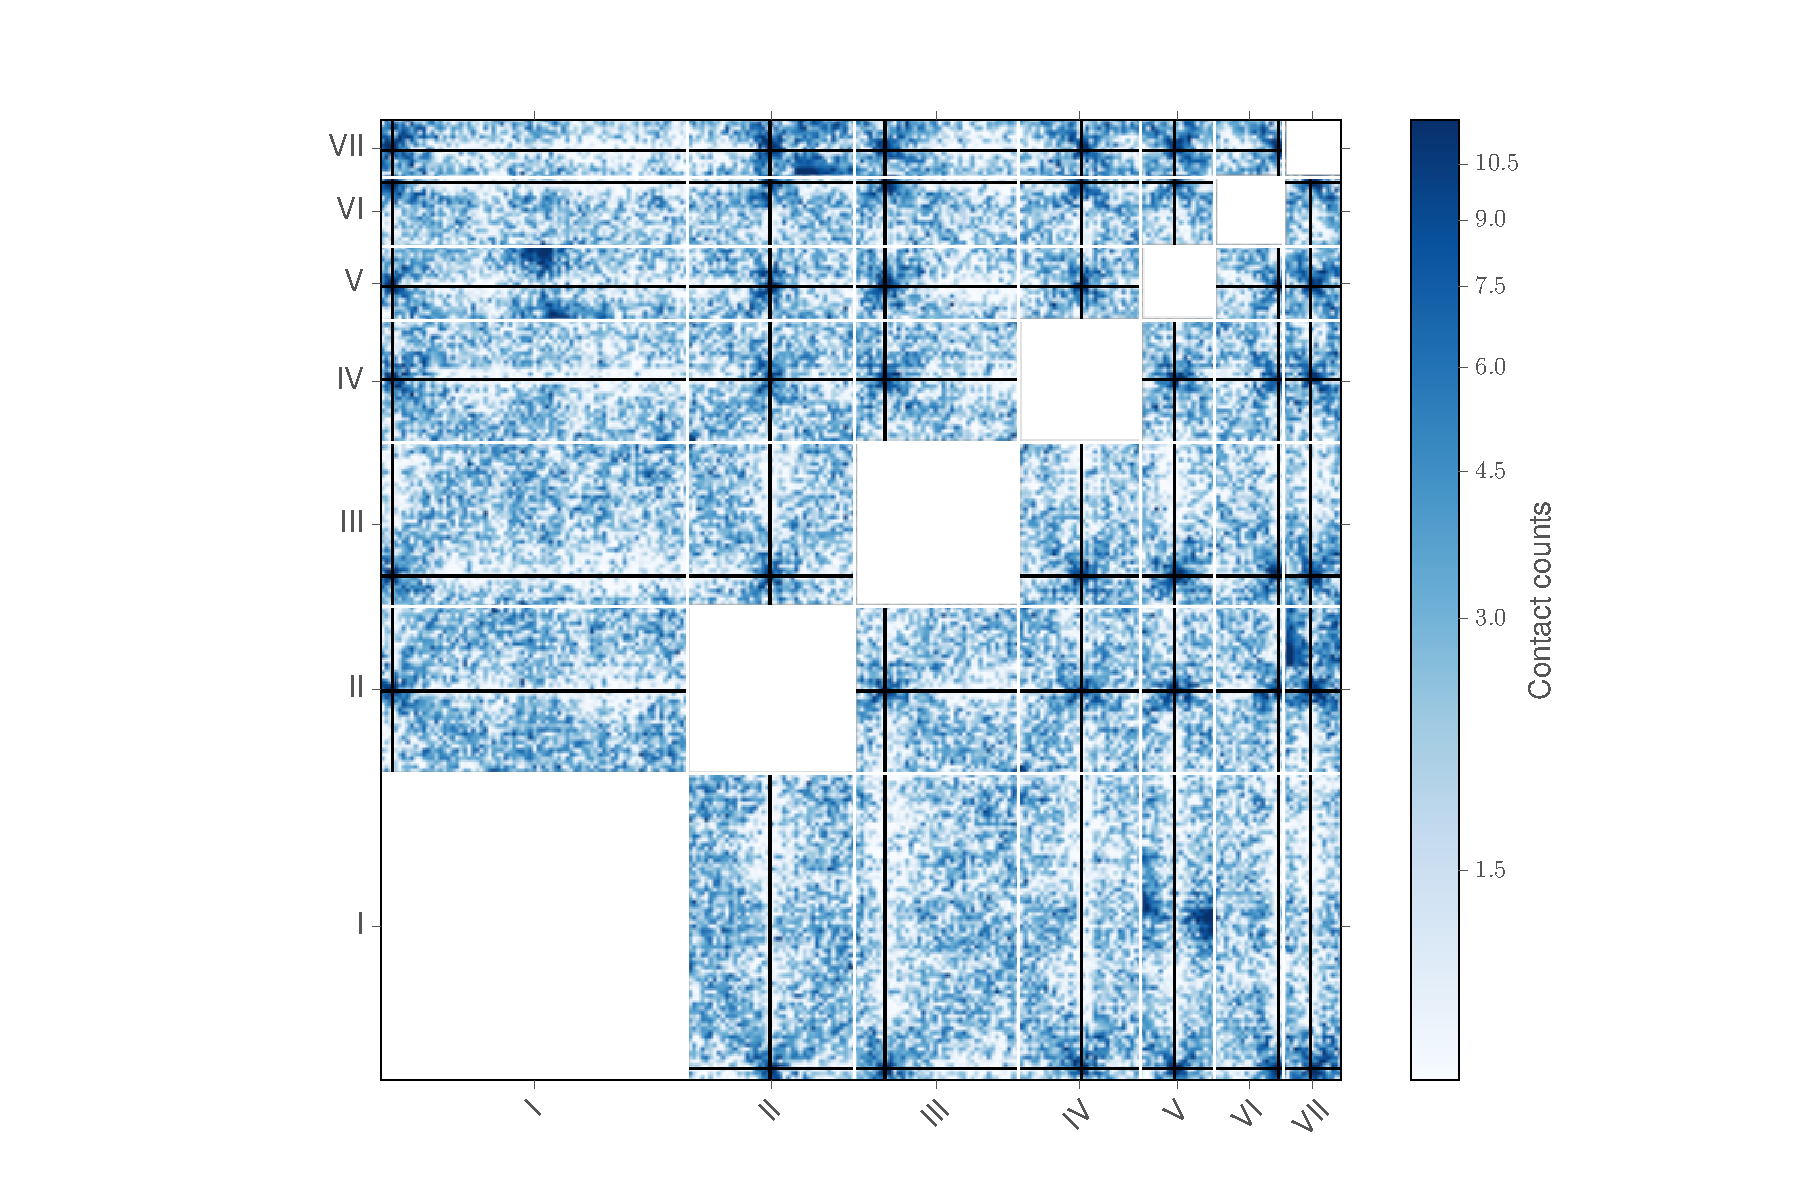
\includegraphics[width=0.9\linewidth]{figures/4_whole_genome_KW.pdf}

\caption{\textbf{\textit{K. wickerhamii}}}
\end{figure}

\end{frame}

\begin{frame}
\frametitle{Conclusion}
\begin{itemize}
\item We propose a method called {\bf Centurion} that jointly infers
centromere locations.
\item Centurion predicts accurate centromere locations and outperforms
existing methods, in particular in high noise settings.
\end{itemize}
\end{frame}

% 7. Conclusion

\section{Conclusion}
\begin{frame}
\begin{center}
\huge{ \bf
Conclusion
}
\end{center}
\end{frame}

% 1. Conclusion

\begin{frame}
\frametitle{Conclusion}
\begin{itemize}[label={$\bullet$}]
\item \textbf{Biological contributions} I
studied the 3D structure of {\em P. falciparum}, which led to a \textit{better
understanding of links between the genome architecture and gene expression and
regulation}.
\item \textbf{\em Methodological contributions}
\begin{itemize}[label={$\bullet$}]
\item development of a stable statistical method for \textit{3D genome
inference}
\item robust and accurate algorithm for \textit{centromere detection in yeast} 
\end{itemize}
\item \textbf{\em Software contributions}: 
\begin{itemize}[label={$\bullet$}]
\item scikit-learn, a machine-learning toolkit written in Python
\item PASTIS
\item Centurion
\item iced, included in HiC-pro
\end{itemize}
\end{itemize}
\end{frame}

\begin{frame}
\frametitle{Perspectives}
\begin{itemize}[label={$\bullet$}]
\item Normalization and Quality Control
\item Inference of 3D models for polyploid genomes
\item Inference of a population of structures using single-cell data
\end{itemize}
\end{frame}


% 2. Acknowledgments
\begin{frame}
\frametitle{Acknowledgments}
\fboxsep=0pt
\noindent
\begin{minipage}[t]{0.48\linewidth}
\textbf{Mines ParisTech - CBIO} \\
Jean-Philippe \textsc{Vert} \\
Thomas \textsc{Walter} \\

\textbf{UW - Noble lab} \\
William S. \textsc{Noble} \\
Ferhat \textsc{Ay} \\

\textbf{Institut Curie - U900} \\
Emmanuel \textsc{Barillot} \\
Nicolas \textsc{Servant} \\
Chong-Jian \textsc{Chen} \\
Eric \textsc{Viara} \\

\textbf{UMass} \\
Job \textsc{Dekker} \\
Bryan \textsc{Lajoie} \\

\end{minipage}
\hfill%
\begin{minipage}[t]{0.48\linewidth}

\textbf{UC Riverside} \\
Karine \textsc{Le Roch} \\
Sebastiaan \textsc{Bol} \\
Evelien \textsc{Bunnik} \\
Jacques \textsc{Prudhomme} \\

\textbf{Institut Curie - UMR168} \\
Edith \textsc{Heard} \\

\textbf{UW - Dunham lab} \\
Maitreya \textsc{Dunham} \\
Ivan \textsc{Liachko} \\

\textbf{UW - Shendure lab} \\
Jay \textsc{Shendure} \\
Josh \textsc{Burton} \\

\end{minipage}

\end{frame}

\begin{frame}[allowframebreaks,noframenumbering]
  \frametitle{References}
  \bibliographystyle{plainnat}
  \bibliography{refs}
\end{frame}

\begin{frame}[noframenumbering]

\end{frame}

\begin{frame}[noframenumbering]
\frametitle{GSEA shows strong enrichments of GO terms in telomeric and
non-telomeric regions}

\begin{table}
\footnotesize
\vspace{10pt}
\begin{center}
\begin{tabular}{lp{0.4\linewidth}ccc}
\hline
\emph{GO term }&  \emph{Description} & \emph{Type} & \emph{Enrichment} &
\emph{q-value}  \\
\hline
GO:0005840 & ribosome & CC & n-t & 0.000\\
GO:0005622 & intracellular & CC & n-t & 0.000\\
GO:0022627 & cytosolic small ribosomal subunit & CC & n-t & 0.000\\
GO:0005789 & endoplasmic reticulum membrane & CC & n-t & 0.000\\
GO:0005783 & endoplasmic reticulum & CC & n-t & 0.000\\
GO:0022625 & cytosolic large ribosomal subunit & CC & n-t & 0.000\\
GO:0015935 & small ribosomal subunit & CC & n-t & 0.000\\
GO:0020002 & host cell plasma membrane & CC & t & 0.000\\
GO:0020030 & infected host cell surface knob & CC & t & 0.000\\
GO:0020036 & Maurer's cleft & CC & t & 0.000\\
GO:0016021 & integral to membrane & CC & t & 0.000\\
GO:0015934 & large ribosomal subunit & CC & n-t & 0.001\\
\dots & \dots & \dots & \dots & \dots \\
\end{tabular}
\end{center}
\end{table}
\end{frame}



\end{document}

